\nonstopmode
\documentclass[10pt,a4paper]{article}
\usepackage[utf8]{inputenc} % para poder usar tildes en archivos UTF-8
\usepackage[spanish]{babel} % para que comandos como \today den el resultado en castellano
\usepackage{a4wide} % márgenes un poco más anchos que lo usual
\usepackage{color}
\usepackage{gnuplottex}
\usepackage{amssymb}
%\usepackage{ccfonts,eulervm}
\usepackage{dot2texi}
\usepackage{tikz}
\usetikzlibrary{shapes,arrows}
\usepackage[T1]{fontenc}
\usepackage{listings}
\usepackage{xcolor}
\usepackage{amsmath}
\lstset { %
    language=C++,
    %backgroundcolor=\color{black!5}, % set backgroundcolor
                   basicstyle=\ttfamily,
                keywordstyle=\color{blue}\ttfamily,
                stringstyle=\color{red}\ttfamily,
                commentstyle=\color{green}\ttfamily,
                morecomment=[l][\color{magenta}]{\#}
}
\usepackage{float}
\usepackage{fancyhdr}
\pagestyle{fancy}
\thispagestyle{fancy}
\addtolength{\headheight}{1pt}
\lhead{AED3}
\rhead{TP3}
\usepackage[ruled,vlined,linesnumbered]{algorithm2e}
\usepackage[conEntregas]{caratula}
\renewcommand*{\algorithmcfname}{Algoritmo}

\begin{document}

\titulo{Trabajo Práctico III}
\subtitulo{Grupo 5}

\fecha{\today}

\materia{Algoritmos y Estructuras de Datos III}

\integrante{Aleman, Damian Eliel}{377/10}{damianealeman@gmail.com}
\integrante{Amil, Diego Alejandro}{68/09}{amildie@gmail.com}
\integrante{Barabas, Ariel}{775/11}{ariel.baras@gmail.com}
\integrante{Fern\'andez, Gonzalo Pablo}{836/10}{ralo4155@hotmail.com}

\maketitle


\tableofcontents

\newpage
\section{Introducción}
\par{El presente informe apunta a documentar el proceso de desarrollo del Trabajo
Práctico número 3 de la materia Algoritmos y Estructuras de Datos III, cursada
correspondiente al segundo cuatrimestre del año 2013.}\\

\par{Este trabajo práctico consiste en el análisis de diferentes heurísticas
para tratar el \emph{Problema de la Clique de Máxima Frontera} (\emph{CMF} de
ahora en más). Dado un grafo $G=(V,E)$, una clique de $G$ es un subconjunto $K$
de los nodos de $V$ tal que para todo par de nodos de $K$, existe una arista
en $E$ que los une. Es decir,}
\[
sea\ G = (V,E),\ K \subseteq V\ es\ clique\ de\ G \Leftrightarrow (v,w)
\in E\ \forall\ v,w \in K
\]

\par{En otras palabras, una clique de $G$ es el conjunto de nodos de un
subgrafo completo de $G$. Dado un conjunto de nodos $C$, se define la frontera
de $C$ en $G$ ($\delta_G$($C$)) como la cantidad de aristas que tienen un
extremo en $C$ y el otro en $V\backslash C$. Es decir,}
\[
sean\ G = (V,E),\ y\ C \subseteq V\ un\ subconjunto\ de\ nodos,\ \delta_G(C)
= |{(v,w) \in E / v \in C \land w \notin C}|
\]

\par{El problema de $CMF$ consiste en, dado un grafo $G$, encontrar
una clique $K$ de $G$ tal que la frontera de $K$ sea mayor a la frontera de
cualquier otra clique de $K$, es decir,}
\[
sean\ G = (V,E),\ y\ K \subseteq V\ una\ clique\ de\ G,\ K\ es\ CMF
\Leftrightarrow \delta_G(K) \geq \delta_G(K')\ \forall K'\ clique\ de\ G
\]

%\par{Exhibimos un ejemplo del problema en la siguiente figura:}

%\textbf{GRAFICO$\_$COPADO.PNG}

%\par{Podemos ver como los vértices coloreados con negro corresponden a la
%clique que tiene la frontera mas grande del grafo, mientras que los coloreados
%con gris corresponden a su frontera.}\\

\par{Para resolver este problema se pide implementar:}
\begin{itemize}
\item Un algoritmo exacto.
\item Una heurística constructiva golosa.
\item Una heurística de búsqueda local.
\item Una metaheurística de búsqueda tabú.
\end{itemize} 

\par{Luego de haber terminado con la programación de nuestras soluciones,
vamos a realizar una experimentación con el objetivo de verificar y comparar
tanto los tiempos de ejecución como los resultados de los programas extrayendo
así conclusiones sobre la performance y la optimalidad de los diferentes
métodos propuestos en este trabajo práctico.}\\

\par{Esperamos, al finalizar este proyecto, tener un entendimiento teórico
sobre el análisis heurístico de problemas difíciles de tratar junto las
herramientas prácticas para poder abordar este tipo de problemas en el futuro.}


\newpage
\section{Pautas de Implementación}
\par{Al igual que en trabajos prácticos anteriores, desarrollaremos
nuestras soluciones en \texttt{C++} y recurriremos a la
\texttt{STL} del mismo de ser necesario. Al igual que en el trabajo práctico
anterior, usaremos una clase grafo propia que representa un grafo mediante
listas de adyacencia y matriz de adyacencia simultáneamente. En el caso de
precisar implementar alguna otra estructura de datos específica vamos a
documentar las características de sus operaciones y adjuntar el código de estas
en el apéndice del código de este informe. Los programas desarrollados se
encuentran en el directorio \texttt{/codigo} dentro del archivo
\texttt{entregable.tar.gz}, los cuales son:}

\begin{itemize}
\item \texttt{exacto/exacto.h} - Contiene la implementación del algoritmo exacto (II).
\item \texttt{goloso/goloso.h} - Contiene la implementación de la heurística golosa (III).
\item \texttt{local/local.h} - Contiene la implementación de la heurística de búsqueda local (IV).
\item \texttt{tabu/tabu.h} - Contiene la implementación de la metaehurística de búsqueda tabú (V).
\item \texttt{timer.h} - Contiene funciones para medir performance.
\item \texttt{grafo.h} - Contiene la clase grafo utilizada en todos los algoritmos.
\end{itemize}

\par{En este directorio también tenemos un \texttt{Makefile} que permite
compilar separadamente cada implementación. De esta manera, si quisiera correr
el algoritmo exacto con los casos de prueba del archivo \texttt{tests.in},
debría compilarlo mediante \texttt{make EXACTO} y luego correrlo escribiendo\\
\texttt{./exacto <  tests.in}.}\\

\par{Para testear los tiempos de ejecución de las
implementaciones contamos con los programas
$test\_exacto$, $test\_goloso$, $test\_local$ y $test\_tabu$ cada uno
en su respectiva carpeta. Cada uno se ejecuta con los parámetros
$N$, $t$ y $s$. Para cada $n$ = $k*s$ ($k$ entero) menor o igual a
$N$, se generan $t$ instancias del problema de tamaño $n$ y se
ejecutan las soluciones implementadas con esas instancias. Luego
se devuelven los resultados obtenidos y los tiempos de ejecución
promedio en función de $n$.}\\

\par{Para testear la optimalidad de las implementaciones contamos con los
programas $opt\_goloso$, $opt\_local$ y $opt\_tabu$ cada uno en su respectiva
carpeta. Estos se ejecutan con los mismos parámetros que sus versiones $test$
asociadas, pero en lugar de devolver los timepos de ejecución, devuelven
lo que llamamos el índice de optimalidad, que nos dice que tan cerca estuvo
el resultado devuelto por la heurística del resultado óptimo. El índice de
optimalidad es un número menor o igual a cero que se calcula como $f$-$O$
con $f$ el valor de la solución devuelta por la heurística y $O$ el valor
de la solución óptima\footnote{A último momento se modificó el índice
de optimalidad para que sea un porcentaje respecto al óptimo en lugar
de ser sólo la diferencia con él.}.}\\

\par{Una instancia del problema de $CMF$ es un grafo cualquiera. La clase
grafo cuenta con 2 constructores: uno sin parámetros que genera un grafo
vacío y otro con un único parámetro $n$ que genera un grafo de $n$ nodos
sin aristas. La función $inicializar$ de la clase $grafo$ toma un grafo vacío
y lo reconstruye a partir de la entrada estándar. La función
$generar\_aristas\_aleatorias$ toma un grafo de $n$ nodos y, por cada posible
arista del grafo (es decir, por cada par de nodos) decide aleatoriamente
si agregarla al grafo o no. La función $generar\_m\_aristas\_aleatorias$
funciona igual pero genera un grafo con exactamente $m$ aristas ($m$ parámetro).}\\

\par{Una solución al problema de $CMF$ es un subconjunto de nodos del
grafo entrada. Para representar una solución utilizaremos una dupla
de un entero y un vector de $n$ booleanos (con $n$ la cantidad de nodos
del grafo). El i-ésimo booleano del vector indica si el i-ésimo nodo del
grafo pertenece a la clique representada por la solución. El entero de la
tupla corresponde al tamaño de la frontera de la solución representada. Notar
que no toda solución representada de esta forma es una solución válida, ya
que no necesariamente representa una clique. A las soluciones que no sean
cliques se les asigna como segundo elemento de la dupla el valor de la
frontera de su subconjunto de nodos\footnote{La frontera no sólo está
definido para cliques sino que lo está para cualquier subconjunto de nodos
de un grafo.}
multiplicado por -$1$, así las soluciones inválidas tendrán
valor de frontera negativo.}


\newpage
\section{Descripción de Situaciones Reales}

\textbf{1 - Invitaciones de Amigos}\\

\par{Aprobamos Algo3, situación digna de un festejo de proporciones descontroladas\footnote{Suponiendo que aprobar Algo3 podría ser una situación de la vida real.}. Como grupo generoso que somos decidimos invitar amigos de nuestra cursada a un boliche para festejar la ocasión.}\\

\par{Este boliche tiene una particularidad: a la zona VIP del mismo sólo pueden entrar grupos de amigos que cumplan la condición de que todos son amigos de todos. El costo de usar la zona VIP es el mismo sin importar cuantos invitados sean. A su vez, el boliche cuenta los martes con la siguiente promoción: si hacemos uso de la zona VIP, entonces el establecimiento nos devuelve a nosotros un porcentaje de cada entrada no-VIP vendida gracias a nuestra invitación.}\\

\par{La pregunta es: ¿Qué grupo de amigos de nuestra cursada de Algo3 deberíamos seleccionar para garantizarnos ganar la mayor cantidad de dinero en esta fiesta}
\\\\
\textbf{2 - Broadcast}\\

\par{Volvemos al segundo ejercicio del Trabajo Práctico 2. En este problema teníamos un servidor denominado $master$ el cual era el encargado de recibir un paquete de información determinado y replicarlo a sus servidores vecinos. Estos servidores vecinos replicarían el mismo paquete a sus vecinos, y así consecutivamente hasta haber copiado el paquete a todos los servidores de la red.}\\

\par{La companía $Algo3 Networking Solutions$ decidió modificar su infraestructura y ahora cuenta también con varios $clusters$. Un $cluster$ es una red de tres o más servidores los cuales están todos conectados entre si. Si un servidor de un determinado $cluster$ recibe un paquete, automáticamente hace un broadcast a todos los otros servidores correspondientes al mismo $cluster$ copiando dicho paquete en todos y luego, cada uno de los servidores del $cluster$ copia el paquete a todos los servidores externos al $cluster$ a los que esté conectado.}\\

\par{No obstante, esta nueva infraestructura cuenta con una desventaja en comparación con la anterior: los únicos servidores que pueden copiar información son los pertenecientes a un $cluster$. El resto sólo puede recibirla.}\\

\par{Lógicamente esto nos presenta un problema: la información puede no ser replicada a todos los servidores. Pero sabemos que si un paquete es transmitido desde un $cluster$ hacia otro $cluster$, este segundo va a poder transmitirla a todos los servidores aislados a los que esté conectado. Si pudiéramos encontrar de alguna manera el $cluster$ que esté conectado a la mayor cantidad de servidores externos a el, estaríamos aumentando las probabilidades de que uno de estos servidores corresponda a otro $cluster$, incrementando el alcance de nuestro paquete.}

\newpage
\section{Algoritmo Exacto}
\subsection{Implementación del Algoritmo}

\par{Para realizar el algoritmo exacto, utilizamos la técnica de programación de
backtracking. Para ver cuál es el clique con una frontera de mayor
cardinalidad, calculamos la frontera de cada clique que hay en el grafo.
Partimos de una solución en la que el conjunto de nodos es vacío\footnote{
Es debatible si esta solución es válida o no, pero al tener frontera igual
a cero, cualquier solución válida con al menos uno de frontera será mejor.
En todo caso, si el grafo no tiene aristas, se devolverá esta solución vacía.}.
Luego utlizamos recursión para agregar cada posible nodo al conjunto. La
función recursiva se llama a sí misma dos veces: una agregando el i-ésimo
nodo a la solución actual y otra sin agregarlo.}\\

\par{A la función recursiva se le pasan como parámetros la solución actual y
la solución óptima hallada hasta el momento (ambas inicializadas con la
solución vacía). Cada vez que se entra a la función recursiva se evalúa el
tamaño de la frontera de la solución actual y si es mayor a la frontera de
la solución óptima, la solución actual reemplaza a la óptima. Una vez
finalizado el algoritmo se retorna la solución almacenada como óptima. La
solución vacía almacenada como óptima será reemplazada en cuanto se evalúe
cualquier solución con tamaño de frontera mayor a cero. Como cada nodo es una
clique, si el algoritmo retorna la solución vacía significa que el grafo no
tiene aristas.}\\

\par{Con el objetivo de reducir la complejidad del algoritmo exacto se ha
implementado una importante poda. Cuando la función va a llamarse
recursivamente, primero se evalúa si tiene sentido agregar el nodo a la
solución actual, es decir si con el nodo que se agrega, la solución actual
sigue representando una clique. Si con ese nodo no se
forma un clique, luego ese subconjunto de nodos sumado a otros nodos, tampoco
va a ser clique. Por esta razón, se poda toda solución que agregue el nodo
a la solución actual, es decir todo subconjunto de nodos, que no forman una
clique. A continuación se muestra un pseudocódigo del algoritmo exacto basado
en backtracking recursivo.}\\

\begin{algorithm}[H]
	\caption{Pseudocódigo del algoritmo exacto}
	\KwData{\textbf{Grafo} $G(V,E)$}
	\textbf{Solucion} $solucion\_optima$ $\leftarrow$ $solucion\_vacia$\\
	\textbf{Solucion} $solucion\_actual$ $\leftarrow$ $solucion\_vacia$\\
	Recursion(0, $solucion\_optima$, $solucion\_actual$)\\
	\textbf{return} $solucion\_optima$
\end{algorithm}

\begin{algorithm}[H]
	\caption{Llamada recursiva}
	\KwData{\textbf{int} $i$, \textbf{Solucion} $solucion\_optima$, \textbf{Solucion} $solucion\_actual$}
	$solucion\_optima$ $\leftarrow$ Max($solucion\_optima$, $solucion\_actual$)\\
	\If{$i$ = $cantNodos$}{
		Terminar recursion
	}

	\eIf{se\_conecta\_con\_clique($i$, $solucion\_actual$)}{
		Agregar $i$ a $solucion\_actual$\\
		Recursion($i+1$, $solucion\_optima$, $solucion\_actual$)\\
		Quitar $i$ de $solucion\_actual$\\
		Recursion($i+1$, $solucion\_optima$, $solucion\_actual$)
	}{
		Recursion($i+1$, $solucion\_optima$, $solucion\_actual$)
	}
\end{algorithm}

\par{La función $Max$ compara dos soluciones y retorna la de mayor frontera.
$cantNodos$ es la cantidad de nodos del grafo. Cuando el índice del nodo que se
va a agregar $i$ es igual a dicha cantidad, significa que ya no hay más nodos
para agregar y la recursión debe terminar. En otras palabras, se llegó a una
hoja del árbol de backtracking. La función $se\_conecta\_con\_clique$ toma un
nodo $i$ y una solución $S$ y retorna si la solución $S$ seguiría representando
una clique tras agregarle el nodo $i$. Para ello evalúa si existe una arista
entre el nodo $i$ y cada nodo de la clique representada por $S$.}

\subsection{Orden de complejidad}

\par{No puede hacerse mucho análisis respecto al orden de complejidad. El
algoritmo exacto recorre todas las posibles soluciones. Si bien hemos
implementado una poda, en el peor caso (un grafo completo $K_n$) todas las
soluciones serán válidas y todas ellas deberán ser evaluadas. Dado que en
una solución cada nodo puede estar o no estar, la cantidad de soluciones
posibles (la cantidad de subconjuntos del conjunto de nodos) es $2^n$ con
$n$ la cantidad de nodos. Las operaciones realizadas para cada solución son
polinomiales y, por lo tanto no aportan a la complejidad exponencial. La
función $se\_conecta\_con\_clique$ compara $k$ elementos con $k$ la cantidad
de nodos del conunto, que es a lo sumo $n$. Cuando se agregan o se quitan
nodos de una solución, la frontera de dicha solución debe recalcularse. La
complejidad de agragar o quitar un nodo $i$ es $d_G(i)$ (el grado de dicho
nodo, que también puede acotarse superiormente por $n$), ya que deben
evaluarse todas sus aristas. En definitiva, la complejidad del algoritmo
exacto es $2^n * ( n + n + n ) \in$ O($2^n$)}

\subsection{Experimentación}

\subsubsection{Performance}

\par{El archivo $test\_exacto.cpp$ en la carpeta $codigo/exacto$ contiene la
implementación del código que mide los tiempos de ejecución del algoritmo
exacto. Se ejecutó este programa con $N$ = 50,\\$s$ = 1 y $k$ = 10. Es decir,
para cada $n$ entero entre 1 y 50, se generaron 10 grafos aleatorios (
con la función $generar\_aristas\_aleatorias$). Para cada instancia generada se
corrieron dos verisones del algoritmo exacto. Uno con la poda y otro sin ella.
En el siguiente gráfico se muestran los resultados obtenidos.}

\begin{center}
\textbf{Gráfico de performance del algoritmo exacto en\\función de la cantidad
de nodos del grafo}
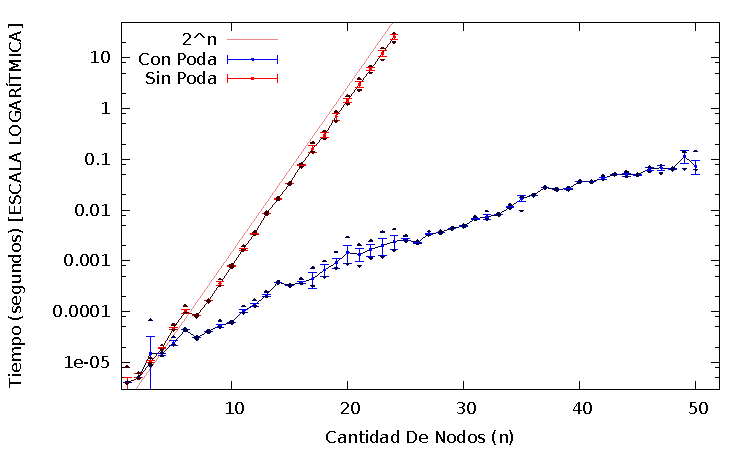
\includegraphics[scale=1.3]{imgs/exacto_50_1_10.pdf}
\end{center}

\par{Cada punto $\bullet$ en el gráfico representa el promedio de los tiempos
medidos para cada una de las 10 ejecuciones de una determinada cantidad de nodos
del grafo. El tamaño del segmento vertical sobre cada punto $\bullet$ representa
su varianza asociada. Además, para cada cantidad de nodos $n$ se graficaron la
máxima medición con $\blacktriangle$ y la mínima medición con
$\blacktriangledown$.}\\

\par{La función graficada con una curva sin puntos es una función exponencial de
base 2. Al estar utilizando escala logarítmica en el eje de ordenadas, esta curva
se ve como una recta. Como se puede observar, la curva definida por la versión
sin poda del algoritmo (la curva resultante de unir los puntos $\bullet$) se
asemeja mucho a tal curva. Mientras que la versión con poda tiene
menores tiempos promedio de ejecución, si bien tiene la misma complejidad.}\\

\par{En la mayotía de los casos, la varianza de ambas versiones es tan pequeña
que apenas puede verse en el gráfico. Esto nos dice que ambas versiones del
algoritmo son estables. Era de esperarse de la versión sin poda, ya que dado
cualquier grafo, la cantidad de soluciones que deben recorrerse es siempre
la misma. Sin embargo, de la versión con poda se esperaba una varianza bastante
superior debido a que la cantidad de soluciones que este debe recorrer depende
en gran medida del grafo entrada.}

\newpage
\section{Heurística Constructiva Golosa}
\subsection{Implementación del Algoritmo}

\par{La heurística golosa consiste en construír una solución por partes. El
algoritmo itera y en cada iteración agrega una parte a la solución. Sea $S$
una solución a un problema dado, llamamos $S_i$ a una subsolución de $S$, es
decir una solución incompleta al problema. Sea $S_i$ = $\{s_1, s_2\dots s_i\}$
la subsolución obtenida en la iteración $i$ de la heurística, y sea $P_i$ =
$\{p_1, p_2\dots p_n\}$ el conjunto de posibles $partes$ de solución tales que
$S_i \cup p_j$ sea también subsolución del problema. Entonces $P_i$ es el
conjunto de candidatos de la iteración $i$. En la iteración $i$, la heurística
golosa debe $elegir$ entre un conjunto $P_i$ de candidatos y una vez
seleccionado el $p_j$ del conjunto, generar una subsolución $S_{i+1}$ compuesta
por $S_i$ y $p_j$. La forma en que se elige el $p_j$ es mediante una función
que le asigna a cada $p_j$ (o a cada $S_i \cup p_j$) un valor numérico. La
heurística golosa elegirá a aquel $p_j$ que maximice dicha función.}\\

\par{En el problema de $CMF$ una solución es un conjunto de nodos. Así que la
heurística golosa implementada construirá el conjunto de nodos solución
agregando un nodo en cada iteración. La función que utilizamos para
seleccionar al mejor candidato (el nodo a agregar) es cuánto incrementaría la
frontera de la solución si se agreagra ese nodo a la solución parcial. Cuando
ningún nodo ampliaría la frontera de la solución parcial (o cuando ya no quedan
nodos que agregar) el algoritmo termina y retorna la solución almacenada. A
continuación se presenta un pseudocódigo de la solución implementada.}\\

\begin{algorithm}[H]
	\caption{Pseudocódigo de la heurística constructiva golosa}
	\KwData{\textbf{Grafo} $G(V,E)$}
	\textbf{Solucion} $solucion\_actual$ $\leftarrow$ $solucion\_vacia$\\
	\While{Puedo agregar nodos}{
		\textbf{int} $candidato$ $\leftarrow$ -1\\
		\textbf{int} $maximo\_aporte$ $\leftarrow$ 0\\
		\For{( \textbf{int} $nodo$ $\in$ $V$, $nodo$ $\notin$ $solucion\_actual$) )}{
			\If{$se\_conecta\_con\_clique$($i$, $solucion\_actual$)}{
				\textbf{int} $aporta$ $\leftarrow$ $cuanto\_aporta(nodo,\ solucion\_actual)$\\
				\If{$aporta >\ maximo\_aporte$}{
					$candidato$ $\leftarrow$ $nodo$\\
					$maximo\_aporte$ $\leftarrow$ $aporta$
				}
			}
		}
		\eIf{$candidato$ = -1}{
			Ya no puedo agregar nodos\\
		}{
			Agregar $candidato$ a $solucion\_actual$\\
		}
	}
	\textbf{return} $solucion\_actual$
\end{algorithm}

\par{Una vez más se inicia con una solución vacía (un conjunto de nodos
vacío). Cualquier nodo con al menos una arista va a sumar a la frontera si
se lo agrega a la solución, por lo que, una vez más el algoritmo devuelve el
conjunto vacío sólo si el grafo no tiene aristas. En cada iteración se
le asigna -1 a la variable $candidato$ la cual contendrá el nodo candidato
a ser agregado a la solución. Luego se itera sobre todos los nodos del grafo
y para cada uno se evalúa cuánto incrementaría la frontera de la solución si
se lo agregara a ella. Si luego de recorrer todos los nodos $candidato$ sigue
valiendo -1, significa que o bien ya todos los nodos están en la solución,
o bien ningún nodo que puede ser agregado aumentaría la frontera de la
solución. Si es ese el caso, se deja de iterar el ciclo principal (línea 2
del pseudocódigo) y se devuelve la $solucion\_actual$.}\\

\par{Luego de iterar sobre todos los nodos, si $candidato$ no vale -1, se
agrega el nodo $candidato$ a la $solucion\_actual$. La función
$se\_conecta\_con\_clique$ retorna si al agregar determinado nodo a una
solución, esta sigue siendo una clique. La función $cuanto\_aporta$
determina cuanto incrementaría (o decrementaría) la frontera de una
solución al agregarle un determinado nodo. Tras iterar sobre todos los
nodos $candidato$ almacena el nodo que más incrementaría el tamaño de la
frontera de la $solucion\_actual$.}

\subsection{Orden de complejidad}

\par{El ciclo prinicipal no puede iterar más de $n$ veces, ya que no se pueden
agreagar más de $n$ nodos a un conjunto de nodos que es subconjunto de los
nodos del grafo. En cada iteración del ciclo principal se recorren todos los
nodos del grafo y, para cada nodo que no pertenece al conjunto se evalúa
cuánto aportaría agregarlo. Dado que el conjunto se representa con un
arreglo de booleanos, ver si el i-ésimo nodo pertenece al conjunto consiste
en evaluar el i-ésimo booleano del arreglo, lo cual se hace en orden constante.
La función $se\_conecta\_con\_clique$\footnote{Tanto esta función como la que
agrega nodos a la solución son las mismas que las utilizadas en el algoritmo
exacto, son funciones declaradas en la clase $grafo$.} tiene complejidad
lineal en la cantidad de nodos del conjunto, la cual puede acotarse
superiormente por $n$.}\\

\par{La función $cuanto\_aporta$, también de la clase $grafo$, calcula
cuánto incrementaría la frontera de la solución agregándole el nodo y
recalculando la frontera de la solución. Hemos visto ya que agregar o quitar
nodos tiene complejidad lineal en el grado del nodo agregado o quitado, el
cual también puede ser acotado superiormente por la cantidad de nodos del
grafo. Finalmente, la complejidad de la heurística constructiva golosa es
$n * ((n * (n+n)) + n) \in$ O($n^3$).}

\subsection{Comportamiento}

\par{En la primera iteración, la heurística agrega a la solución el nodo
de mayor grado. Dado que se parte del conjunto vacío, cualquier nodo
puede ser agregado a la solución y formará una clique de un nodo, en el
que la frontera sea la cantidad de aristas que inciden sobre el nodo. Con
esto podemos afirmar que la heurística golosa encuentra la solución óptima
en grafos estrella\footnote{Un grafo con un nodo central y el resto de los
nodos unidos únicamente al nodo central, es decir un bipartito $K_{1n}$} o
en grafos cuyas componentes conexas son todas estrellas.}\\

\par{Esto también nos da una cota inferior al resultado devuelto por la
heurística. Dado que, una vez obtenida una solución, sólo se agregan nodos
si hacerlo mejora la solución, entonces la heurística golosa nunca devolverá
una solución con frontera menor al grado máximo del grafo. Sin embargo, esto
no nos dice que tan cerca puede estar de la solución óptima, ya que la frontera
de la $CMF$ puede ser tanto mayor al grado máximo como uno quiera.}\\

\par{Por ejemplo, un grafo $G$ con una componente conexa que es una estrella
de $\Delta$($G$)+1 nodos (con $\Delta$($G$) el grado máximo del grafo $G$) y
otra componente conexa de dos nodos adyacentes, cada uno adyacente a
otros $\Delta$($G$)-2 nodos. La heurística tomaría como primer nodo el centro
de la estrella que es adyacente a $\Delta$($G$) nodos y esa es la frontera de
la solución. En la segunda iteración, evaluaría agregar alguno de los nodos
adyacentes al centro de la estrella, pero no lo haría por que todos ellos
reducirían en 1 la frontera obtenida hasta el momento. Entonces la heurística
devolvería este nodo como $CMF$ cuando existe una clique de dos nodos con
frontera 2*($\Delta$($G$)-2) =\\2*$\Delta$($G$) - 4 nodos, que claramente es
mayor (para valores de $\Delta$($G$) suficientemente grandes) a $\Delta$($G$).
La diferencia entre la frontera de la solución golosa y la de la $CMF$ es\\
2*$\Delta$($G$) - $\Delta$($G$) - 4 = $\Delta$($G$) - 4, y puede crecer
tanto como uno quiera aumentando el valor de $\Delta$($G$).}

\subsection{Experimentación}

\subsubsection{Performance}

\par{El archivo $test\_goloso.cpp$ en la carpeta $codigo/goloso$ contiene la
implementación del código que mide los tiempos de ejecución de la heurística
golosa. Se ejecutó este programa con $N$ = 3000, $s$ = 50 y $k$ = 10. Es decir,
para cada $n$ entero múltiplo de 50, entre 50 y 3000, se generaron 10 grafos
aleatorios (con la función $generar\_aristas\_aleatorias$). Para cada instancia
generada se corrió la heurística golosa.
En el siguiente gráfico se muestran los resultados obtenidos.}

\begin{center}
\textbf{Gráfico de performance de la heurística golosa en\\función de la cantidad
de nodos del grafo}
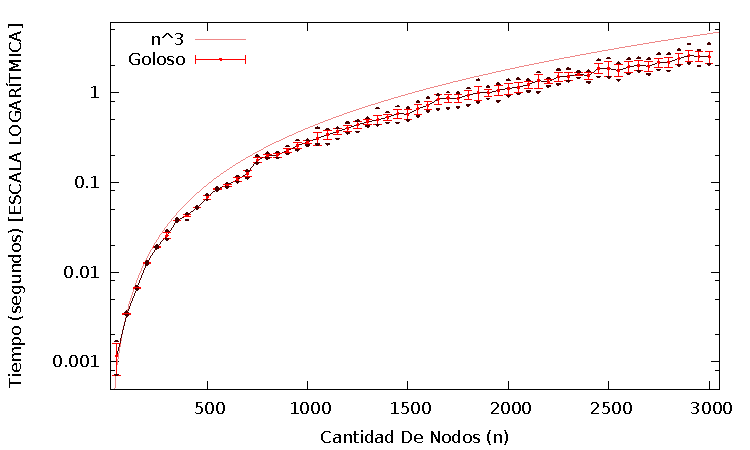
\includegraphics[scale=1.3]{imgs/goloso_3000_50_10.pdf}
\end{center}

\par{Cada punto $\bullet$ en el gráfico representa el promedio de los tiempos
medidos para cada una de las 10 ejecuciones de una determinada cantidad de nodos
del grafo. El tamaño del segmento vertical sobre cada punto $\bullet$ representa
su varianza asociada. Además, para cada cantidad de nodos $n$ se graficaron la
máxima medición con $\blacktriangle$ y la mínima medición con
$\blacktriangledown$.}\\

\par{La función graficada con una curva sin puntos es una función cúbica. Al
estar utilizando escala logarítmica en el eje de ordenadas, esta curva
se ve cóncava. Como se puede observar, la curva definida por la heurística
(la curva resultante de unir los puntos $\bullet$) se asemeja mucho a tal
curva.}

\subsubsection{Optimalidad}

\par{El archivo $opt\_goloso.cpp$ en la carpeta $codigo/goloso$ contiene la
implementación del código que mide el índice de optimalidad de la heurística
golosa. Se ejecutó este programa con $N$ = 100\footnote{Para el test
de performance ejecutamos instancias de tamaño 3000. Sin embargo, para calcular
la optimalidad de la heurísica también debemos ejecutar el algoritmo exacto
con cada instancia, lo que nos restringe el máximo tamaño de entrada.},
$s$ = 1 y $k$ = 10. Es decir, para cada $n$ entero entre 1 y 100, se
generaron 10 grafos aleatorios (con la función $generar\_aristas\_aleatorias$).
Para cada instancia generada se corrió la heurística golosa.
En el siguiente gráfico se muestran los resultados obtenidos.}
\newpage
\begin{center}
\textbf{Gráfico de optimalidad de la heurística golosa en función\\de la cantidad
de nodos del grafo}
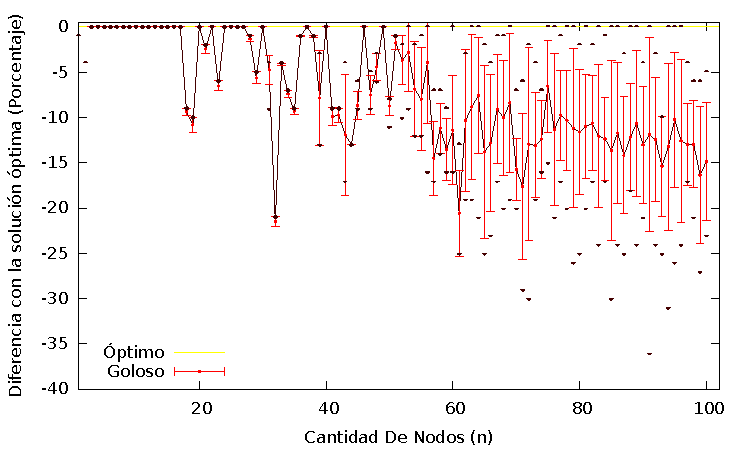
\includegraphics[scale=1.3]{imgs/opt_goloso_100_1_10.pdf}
\end{center}

\par{Cada punto $\bullet$ en el gráfico representa el promedio del índice de
optimalidad para cada una de las 10 ejecuciones de una determinada cantidad de
nodos del grafo. El tamaño del segmento vertical sobre cada punto $\bullet$
representa su varianza asociada. Además, para cada cantidad de nodos $n$ se
graficaron la máxima medición con $\blacktriangle$ y la mínima medición con
$\blacktriangledown$.}\\

\par{La recta $y=0$ representa la solución óptima, así que cuanto más se
asemeje la curva definida por la heurística a dicha recta, mejor es la
heurística. Como se puede observar, para pequeños valores de $n$ la heurística
encuentra siempre, o casi siempre, una solución óptima. Al aumentar la cantidad
de nodos, aumentan tanto la diferencia respecto a la solución óptima, como la
varianza asociada.}\\

\par{Incluso para $n$ mayores, hay instancias para las que la
heurística encuentra una solución óptima. Esto se ve en los $\blacktriangle$
que están sobre la curva $y=0$. Aunque para los mismos $n$ hay instancias en
que la solución devuelta difiere en más del 30\% del óptimo. Como esperábamos,
la varianza en el índice de optimalidad de la heurística es muy grande debido
a que este depende mucho del tipo de grafo que resuelve. Al incrementar la
cantidad de nodos, la curva definida por los resultados del algoritmo
parece estabilizarse. En promedio la heurística golosa parece encontrar
soluciones que representan al rededor del 15\% del óptimo. También parece
no ser peor del 40\%.}\\

\par{Para demostrar que la cota inferior deducida en la sección
\textbf{Comportamiento} es correcta, se realizó otro porgrama que mide el
índice de optimalidad, pero esta vez en lugar de calcular el promedio,
devuelve el valor para cada instancia, además del valor del grado máximo de
cada instancia. El programa está implementado en el archivo $cota\_goloso$ en
la carpeta $codigo/goloso$ y se ejecutó con los mismos parámetros.
En el siguiente gráfico se muestran los resultados obtenidos.}
\newpage
\begin{center}
\textbf{Gráfico de optimalidad de la heurística golosa en función\\de la cantidad
de nodos del grafo (comparación con el grado máximo)}
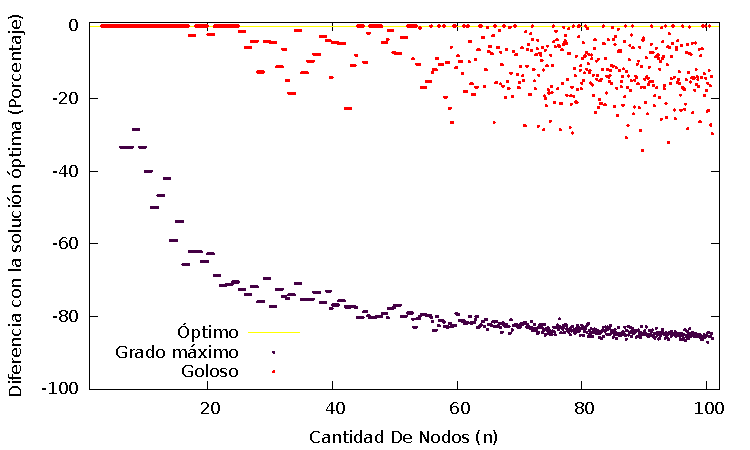
\includegraphics[scale=1.3]{imgs/cota_goloso_100_1_10.pdf}
\end{center}

\par{Cada punto $\bullet$ rojo en el gráfico representa el índice de
optimalidad de una de las 10 instancias de una determinada cantidad de
nodos del grafo. Cada punto $\bullet$ morado representa, para la misma
instancia la diferencia entre el grado máximo del grafo y el valor de una
solución óptima (en procentaje). Para que no se superpongan los puntos
correspondientes a un mismo $n$, la coordenada $x$ de cada punto
no está exactamente sobre $x=n$, sino que está un poco corrido. Como se puede
observar, para cada instancia del problema, el valor de la solución devuelta
por la heurística es mayor o igual al grado máximo del grafo entrada.}

\newpage
\section{Heurística de Búsqueda Local}
\subsection{Implementación del Algoritmo}

\par{La heurística de búsqueda local consiste en tomar una solución cualquiera
al problema, la solución inicial y mejorarla a través de sucesivas iteraciones.
En cada iteración, en base a la solución actual que se recorre, se construye un
conjunto acotado de soluciones, del que se elige la mejor, la cual pasará a
ser la nueva solución actual. Cuando ninguna de las soluciones de dicho
conjunto es mejor que la solución actual, la heurística termina, ya que alcanzó
un máximo local.}\\

\par{Dada una solución $S$ se define la vecindad de
la solución $S$ como el conjunto de soluciones $similares$ a la solución $S$
o que tienen algo en común con $S$. La función que construye la vecindad de
una solución es la parte más importante de la heurística. En un extremo, la
función podría hacer que todas las soluciones sean vecinas entre sí, por lo que
partiendo de cualquier solución inicial, en una sola iteración se encontraría
la solución óptima, a costas de tener que recorrer todas las posibles
soluciones al problema. En el otro extremo, la vecindad podría ser tan pequeña
que se alcance un óptimo local en una solución muy lejana al óptimo global, ya
que todas sus vecinas serían menores a ella.}\\

\par{En el problema de $CMF$ una solución se representa con un vector de
booleanos donde el i-ésimo elemento del vector inidica si el i-ésimo nodo
del grafo pertenece al conjunto representado por la solución. Para la
implementación de esta heurística se definió la vecindad de una solución $S$
como el conjunto de soluciones que se pueden formar agregándole o quitándole
nodos a la solución $S$. Dado que una solución representa una clique de un
grafo, quitarle nodos a una solución siempre genera una solución válida (al
quitarle nodos a una clique, sigue siendo una clique). Sin embargo, agregarle
nodos a una clique no necesariamente genera otra clique, por lo que no todas
las soluciones vecinas de una solución válida son válidas.}\\

\par{Dada una solución $S$, el conjunto de soluciones vecinas de $S$ se genera
alternando los valores booleanos de una determinada cantidad $V$ de elementos
de $S$. Llamaremos tamaño de la vecindad a ese valor $V$. Las soluciones
pertenecientes a una vecindad de $S$ de tamaño $V$ son aquellas que se pueden
formar alternando \textbf{a lo sumo} $V$ valores booleanos de $S$. Entonces,
la cantidad de elementos pertenecientes a una vecindad de tamaño $V$ es}

\[
n + \binom{n}{2} + \binom{n}{3} + \dots + \binom{n}{V} = \sum_{i=1}^{V} \binom{n}{i}
\]

\par{Notar que el valor del tamaño de la vecindad $V$ no es la cantidad de
elementos de la vecindad. El valor $V$ es pasado como parámetro de la
implementación. Una valor mayor de $V$ producirá vecindades de mayor
cardinalidad, aumentando la complejidad del algoritmo, pero también
impulsando que se converga más rápido a la solución óptima. Notar que
al utilizar la cantidad de nodos $n$ del grafo como tamaño de vecindad
se está produciendo una instancia en la que todas las soluciones son vecinas
entre sí. Esto quiere decir que en una sola iteración se alcanzará la
solución óptima pero la complejidad es la de evaluar todas las soluciones
posibles, es decir es la complejidad de un algoritmo exacto:}
\[
\sum_{i=1}^{n} \binom{n}{i} = 2^n -1
\]
\par{La estructura básica de la implementación respeta el pseudocódigo estándar
del algoritmo de búsqueda local, sólo que en lugar de generar un conjunto de
soluciones vecinas y luego recorrerlas, las soluciones se van generando a
medida que se recorre la vecindad. Esto permite, mientras se generan las
soluciones de la vecindad, comprobar la validez de las mismas y calcular
la frontera de cada solución vecina a partir de la frontera de la solución
actual, sin tener que guardarlas todas. A continuación se muestra el
pseudocódigo de la heurística.}\\

\begin{algorithm}[H]
	\caption{Pseudocódigo de la heurística de búsqueda local}
	\KwData{\textbf{Grafo} $G(V,E)$, \textbf{Solucion} $solucion\_inicial$}
	\textbf{Solucion} $solucion\_actual$ $\leftarrow$ $solucion\_inicial$\\
	\While{No se alcance un máximo local}{
		\textbf{Solucion} $mejor$\\
		\For{( \textbf{Solucion} $temporal$ $\in$ Vecindad($solucion\_actual$) )}{
			$mejor$ $\leftarrow$ Max($mejor$, $temporal$)
		}
		$solucion\_actual$ $\leftarrow$ $mejor$\\
	}
	\textbf{return} $solucion\_actual$
\end{algorithm}

\par{En la variable $solucion\_actual$ se guarda la solucion que se está
recorriendo. Esta se inicializa con la $solucion\_inicial$ y, en cada
iteración del ciclo principal (línea 2 del pseudocódigo) se reemplaza por la
mejor de sus vecinas, siempre y cuándo, esta sea mejor que la
$solucion\_actual$. Si no lo es, quiere decir que el mejor vecino de la
$solucion\_actual$ tiene menor frontera que ella, en otras palabras, se
ha alcanzado un máximo local. En dicho caso, el ciclo termina y el algoritmo
retorna la solución almacenada en $solucion\_actual$.}\\

\par{Para determinar la mejor entre dos soluciones se utiliza la función $Max$,
la cual obtiene el tamaño de la frontera de las soluciones que compara. A las
soluciones inválidas (que no representan cliques en el grafo) se les asigna
un valor negativo, para que no puedan ser elegidas como $mejor$, a menos claro
que todas las soluciones vecinas sean inválidas. Sin embargo, no se corren
riesgos de devolver una solución inválida, ya que la $solucion\_actual$ se
inicializa con la $solucion\_inicial$ que se asume válida (y por lo tanto con
frontera mayor o igual a cero) y $solucion\_actual$ solo se actualiza con
soluciones mejores (estrictamente) que ella.}

\subsection{Orden de complejidad}

\par{El ciclo principal itera $\#i$ veces. Luego recorre los $\#v$ elementos de
la vecindad de la\\$solucion\_actual$. En el archivo $grafo.h$ se define la
función $obtener\_vecino$ que retorna un elemento de la vecindad. Esta
función toma la solución $S$ y alterna (quita o saca) hasta $V$ nodos de $S$.
El tamaño de la frontera de la solución vecina se recalula en base a los
nodos alternados respecto a $S$. Para cada nodo alternado, deben obtenerse
tadas las aristas que inciden sobre él y evaluar si estas pasan a pertenecer
a la frontera de $S$, o dejan de estarlo. Esto se repite para cada nodo que
se alterna y son a lo sumo $V$, por lo que la complejidad de la función
$obtener\_vecino$ es $V*\Delta(G)$ con $\Delta(G)$ el grado máximo del grafo
de entrada $G$, el cual pertenece al orden de la cantidad de nodos $n$.}\\

\par{Para cada elemento de la vecindad de $S$, se comparan
linealmente los tamaños de la frontera entre él y otras soluciones. En cada
iteración del ciclo principal el valor de frontera de la $solucion\_actual$
incrementa en, al menos uno. Este se inicializa con la frontera de la
solución inicial, aunque podría ser cero. El máximo valor que puede tomar la
frontera de la $solucion\_actual$ es $m$ y el ciclo principal itera hasta que
esa frontera no puede mejorar, es decir que itera a lo sumo $m$ veces.}\\

\par{Esta cota es muy poco ajustada, ya que sólo podría darse
con un grafo que tenga una clique cuya frontera sea todas las aristas del
grafo. En dicho caso, la clique solución no podría contener aristas y por lo
tanto sería un solo nodo adyacente a todos los demás, en otras palabras, una
estrella. Pero si fuese ese el caso, entonces no sería posible que la frontera
de la $solucion\_actual$ tome todos los valores intermedios entre 1 y m-1,
ya que no existen cliques con fronteras de esos tamaños, exepto claro
en estrellas de menos de 4 aristas. También hay que tener en cuenta que
se parte de una solución inicial (aunque su valor de frontera podría ser
cero), por lo que una cota más ajustada es $(m-f_i)$ con $f_i$ el tamaño de
frontera de la solución inicial, la cual sigue siendo del orden de $m$.}

\par{En conclusión, la complejidad del algoritmo es O($m * \#v * V*\Delta(G)$).
Como se mencionó anteriormente, la cantidad de elementos $\#v$ de una vecindad
de tamaño $V$ es}
\[
\sum_{i=1}^{V} \binom{n}{i}
\]

\par{Llamaremos $F(V)$ a dicha función. $F(V)$ puede ser acotada superiormente
por $2^n$ para cualquier $V$, ya que el máximo valor de $V$ es la cantidad de
nodos $n$ (no tendría sentido que fuese mayor) y, con dicho valor el resultado
de la ecuación anterior es $2^{n-1}$. Sin embargo, no tiene sentido utilizar
una vecindad tan grande, la idea es que el tamaño de la vecindad $V$ no sea
mucho mayor a 1. En los siguientes gráficos se ve que, dada una cantidad de
nodos $n$ fija, la complejidad de $F(V)$ es del orden de $2^n$.}

\begin{center}
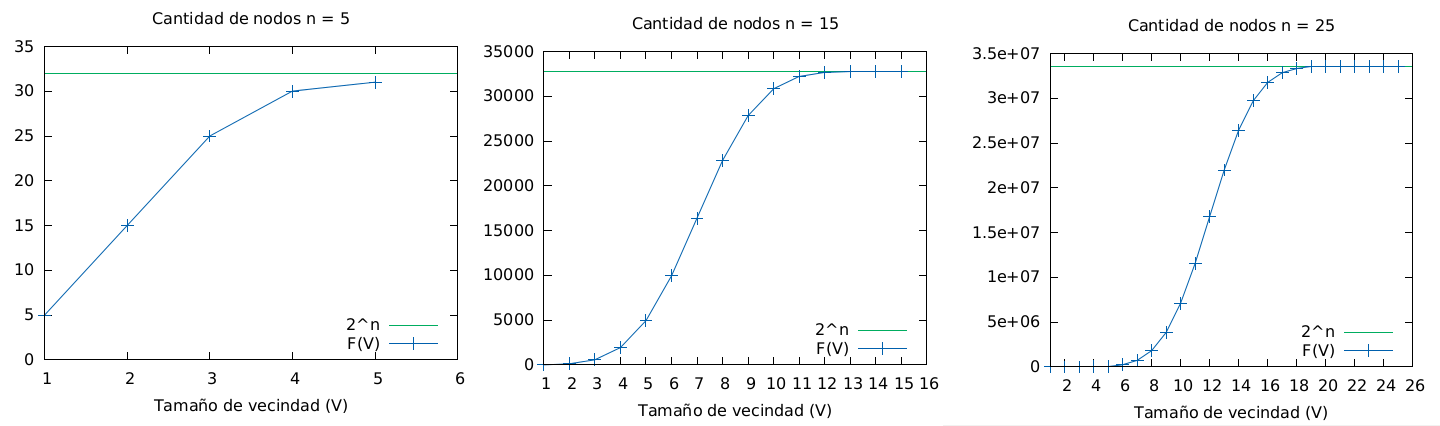
\includegraphics[scale=0.32]{imgs/v.png}
\end{center}

\par{Al incrementar el $n$, son más los valores de $V$ para los cuales $F(V)$
es insignificante frente a la complejidad de $2^n$. Si bien es cierto que $V$
podría tomar valores hasta al rededor de $n/5$ sin alterar la complejidad del
algoritmo, se espera que los valores utilizados no sean mayores a $3$,
incluso para valores de $n$ mucho más grandes. Es por esto que se considerará
la complejidad en función de $V$ con $F(V)$, si bien es cierto que, formalmente,
esta complejidad está acotada superiormente por $2^n$.}\\
 
\par{Finalmente, la complejidad de la implementación de búsqueda local es\\
$(m-f_i) * F(V) * V*\Delta(G) \in$ O($m*2^n*n$). Si bien esta
complejidad parece excesiva para una heurística (de hecho es mayor a la
complejidad de evaluar todas las soluciones), hay dos razones que nos llevan a
pensar que en la práctica se comportará mejor. En primer lugar, deben tomarse
instancias muy específicas (o parámetros muy malos) para que la cantidad de
iteraciones se acerque a $m$. Es esperable que, de haber muchas soluciones
vecinas mejores, se consiga una de frontera varias
veces mayor a la actual y no necesariamente mejorar siempre de a uno, con
lo cual, la cantidad de iteraciones estaría lejos del valor de $m$.}\\

\par{En segundo lugar, la elección del parámetro $V$.
Con un tamaño de vecindad de $V = 1$, la cantidad de vecinos de cada solución es
$F(1) = \binom{n}{1} = n$ la cual es una buena cantidad de vecinos y
resulta en una complejidad de O($m*n*n$). La cantidad de aristas $m$ se puede
acotar por $n^2$ con lo que la complejidad sería $n^2 * n * n \in$
O($n^4$), es decir, es polinomial. Incluso si $V$ fuese 2 o 3 los tiempos
de ejecución tampoco se acercarían a la complejidad del algoritmo exacto.}

\subsection{Comportamiento}

\par{El índice de optimalidad (que tan cercana a la solución óptima es la
solución devuelta) de la heurística de búsqueda local depende mucho del
parámetro $V$, así como de la solución inicial. Si la solución inicial
es una tal que todas sus vecinas son peores (estrictamente) que ella, el
algoritmo no mejorará la solución y devolverá la solución inicial. Como ya se
mencionó, una vecindad muy pequeña tiene más posibilidades de estancarse en
un óptimo local cuando en la misma instancia una vecindad mayor permitiría
alcanzar soluciones mejores.}\\

\par{La única cota inferior a la frontera de la solución devuelta por esta
heurística es la frontera de la solución inicial, la cual puede diferir de la
frontera de la solución óptima tanto como uno quiera. En grafos con grados
pequeños, la heurística tiene mayores posibilidades de encontrar una solución
óptima. De hecho, si se ejecuta el algoritmo con $V$ = $\Delta$($G$) y la
solución inicial igual al conjunto vacío, la vecindad de la solución inicial
en la primera iteración incluirá todas las posibles cliques del grafo, es decir
que en una sola iteración obtendrá la solución óptima. Cuando $\Delta$($G$) es
demasiado grande, no tiene sentido hacer eso, ya que la complejidad superaría
la del algoritmo exacto.}

\subsection{Experimentación}

\subsubsection{Performance}

\par{El archivo $test\_local.cpp$ en la carpeta $codigo/local$ contiene la
implementación del código que mide los tiempos de ejecución de la heurística
de búsqueda local. Se ejecutó este programa con $N$ = 1200, $s$ = 20 y $k$ = 10.
Es decir, para cada $n$ entero múltiplo de 20, entre 20 y 1200, se generaron
10 grafos aleatorios (con la función $generar\_aristas\_aleatorias$). Para cada
instancia generada se corrieron tres versiones de la heurística de búsqueda
local. Con V=1, con V=2 y con V=3. Para las tres, la solución inicial fue la
solución vacía.
En el siguiente gráfico se muestran los resultados obtenidos.}

\begin{center}
\textbf{Gráfico de performance de la heurística de búsqueda local\\ en
función de la cantidad de nodos del grafo}
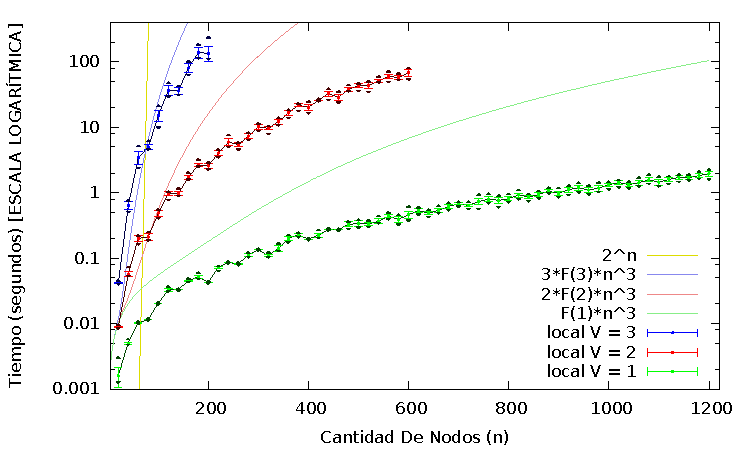
\includegraphics[scale=1.3]{imgs/local_1200_20_10.pdf}
\end{center}

\par{Cada punto $\bullet$ en el gráfico representa el promedio de los tiempos
medidos para cada una de las 10 ejecuciones de una determinada cantidad de nodos
del grafo. El tamaño del segmento vertical sobre cada punto $\bullet$ representa
su varianza asociada. Además, para cada cantidad de nodos $n$ se graficaron la
máxima medición con $\blacktriangle$ y la mínima medición con
$\blacktriangledown$.}\\

\par{La función graficada con una curva amarilla es una función exponencial de
base 2. Al estar utilizando escala logarítmica en el eje de ordenadas, esta curva
se ve como una recta. También se graficaron otras tres funciones para que acoten
superiormente cada una de las heurísticas, basándose en su complejidad estimada
en función de $F(V)$. Como se puede observar, si bien incrementando el $V$ los
tiempos de ejecución de la heurística aumentan considerablemente, están muy
lejos de asemejarse a la curva de la función exponencial\footnote{Para que
las comparaciones tengan sentido, las cuatro funciones graficadas fueron
multiplicadas por las mismas constantes. Es por ello que fue difícil ajustar
las tres cotas superiores a las curvas definidas por las tres heurísticas.},
la cual se ve en el gráfico como una recta casi vertical.}

\subsubsection{Optimalidad}

\par{El archivo $opt\_local.cpp$ en la carpeta $codigo/local$ contiene la
implementación del código que mide el índice de optimalidad de la heurística
de búsqueda local. Se ejecutó este programa con $N$ = 100\footnote{Para el test
de performance ejecutamos instancias de tamaño 1200. Sin embargo, para calcular
la optimalidad de la heurísica también debemos ejecutar el algoritmo exacto
con cada instancia, lo que nos restringe el máximo tamaño de entrada.},
$s$ = 2 y $k$ = 10. Es decir, para cada $n$ entero par entre 2 y 100, se
generaron 10 grafos aleatorios (con la función $generar\_aristas\_aleatorias$).
Para cada instancia generada se corrieron las mismas tres versiones de la
heurística de búsqueda local. Para las tres, la solución inicial fue la
solución vacía. Para que los datos no se amontonen, utlizamos $s$ = 2 en lugar
de\\$s$ = 1.
En el siguiente gráfico se muestran los resultados obtenidos.}

\begin{center}
\textbf{Gráfico de optimalidad de la heurística de búsqueda local\\
en función de la cantidad de nodos del grafo}
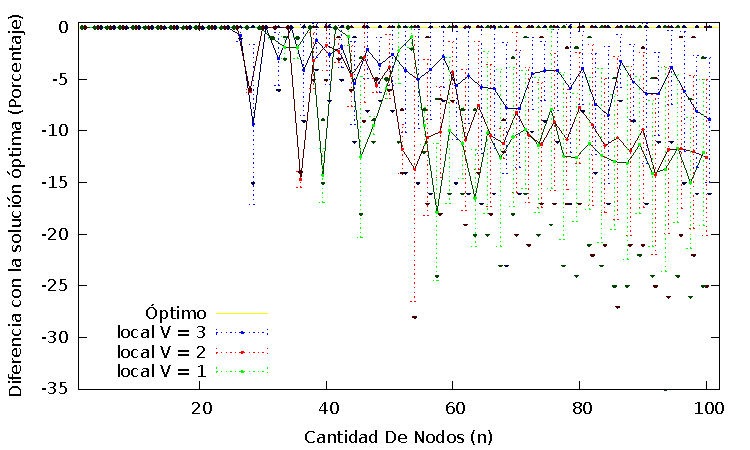
\includegraphics[scale=1.3]{imgs/opt_local_100_2_10.pdf}
\end{center}

\par{Cada punto $\bullet$ en el gráfico representa el promedio del índice de
optimalidad para cada una de las 10 ejecuciones de una determinada cantidad de
nodos del grafo. El tamaño del segmento vertical (en líneas punteadas, también
para que los datos no se amontonen) sobre cada punto $\bullet$
representa su varianza asociada. Además, para cada cantidad de nodos $n$ se
graficaron la máxima medición con $\blacktriangle$ y la mínima medición con
$\blacktriangledown$.}\\

\par{La recta $y=0$ representa la solución óptima, así que cuanto más se
asemeje la curva definida por una heurística a dicha recta, mejor es la
heurística. Como se puede observar, para pequeños valores de $n$ las tres
variantes de la heurística encuentran siempre, o casi siempre, una solución
óptima. Al aumentar la cantidad de nodos, aumentan tanto la diferencia
respecto a la solución óptima, como la varianza asociada.}\\

\par{Como esperábamos, los resultados obtenidos por la variante con $V$=3 son
mejores a los obtenidos por las otras dos variantes. Sin embargo no se ve una
mejora considerable por parte de la variante con $V$=2 respecto a la variante
con $V$=1, de hecho es peor en algunos casos.}\\

\par{Incluso para $n$ mayores, hay instancias para las que las
heurísticas encuentran una solución óptima. Esto se ve en los $\blacktriangle$
que están sobre la curva $y=0$. Aunque para los mismos $n$ hay instancias en
que las soluciones devueltas por las variantes con $V$=1 y $V$=2 difieren en
más del 25\% del óptimo. No es así con la variante con $V$=3, cuyos mínimos en
dichos casos difieren en al rededor del 15\% respecto a la solución óptima y tiene
más casos en los que encuentra una solución óptima, que las otras dos variantes.
Como esperábamos, la varianza en el índice de optimalidad de la heurística
es muy grande debido a que este depende mucho del tipo de grafo que resuelve.
Al incrementar la cantidad de nodos, las curvas definidas por los resultados de
los algoritmos parecen estabilizarse. En promedio la variante con $V$=3 parece
encontrar soluciones que representan entre el 5\% y el 10\% del óptimo, mientras
que las otras dos variantes parecen estabilizarse entre el 10\% y el 15\%.
También parece que ninguna de las tres variantes es peor del 35\%.}

\newpage
\section{Heurística de Búsqueda Tabú}
\subsection{Implementación del Algoritmo}

\par{La implementación de la heurística de búsqueda tabú es muy similar a la
implementación de la heurística de búsqueda local. La vecindad se definió
de la misma forma (con $V$ como parámetro). Al pseudocódigo de búsqueda local
se le agregó todo lo referente a la lista tabú, además de la definición de un
criterio de terminación. A continuación se muestra el pseudocódigo de la
heurística.}\\

\begin{algorithm}[H]
	\caption{Pseudocódigo de la heurística de búsqueda tabú}
	\KwData{\textbf{Grafo} $G(V,E)$, \textbf{Solucion} $solucion\_inicial$}
	\textbf{Solucion} $solucion\_optima$ $\leftarrow$ $solucion\_inicial$\\
	\textbf{Solucion} $solucion\_actual$ $\leftarrow$ $solucion\_inicial$\\
	\While{No se alcance el criterio de terminación}{
		\textbf{Solucion} $mejor$\\
		\For{( \textbf{Solucion} $temporal$ $\in$ Vecindad($solucion\_actual$) )}{
			$solucion\_optima$ $\leftarrow$ Max($solucion\_optima$, $temporal$)\\
			\If{$\neg$EsTabu($temporal$)}{
				$mejor$ $\leftarrow$ Max($mejor$, $temporal$)
			}
		}
		EsTabu($solucion\_actual$)\\
		$solucion\_actual$ $\leftarrow$ $mejor$\\
	}
	\textbf{return} $solucion\_optima$
\end{algorithm}

\par{La variable $solucion\_optima$ guarda la mejor solución encontrada hasta
el momento. La variable $solucion\_actual$ guarda la solución sobre la que se
está iterando. Mientras no se alcance el criterio de terminación, se recorre
toda la vecindad de la $solucion\_actual$. Para cada solución vecina, se
evalúa si es mejor que la $solucion\_optima$ hallada hasta el momento. Si lo
es, la reemplaza. Luego se evalúa si es un candidato a ser la próxima
$solucion\_actual$. Para ello debe ser mejor que la $mejor$ vecina de la
$solucion\_actual$. Si lo es y no es una solución tabú, pasa a ser la nueva
$mejor$. Una vez obtenida la $mejor$ solución vecina de $solucion\_actual$,
se agrega a $solucion\_actual$ a la lista tabú, para no volver a caer en ella
y se le asigna a $solucion\_actual$ el valor de la solución vecina $mejor$.}\\

\par{Para determinar la mejor entre dos soluciones se utiliza la función $Max$,
la cual obtiene el tamaño de la frontera de las soluciones que compara. A las
soluciones inválidas (que no representan cliques en el grafo) se les asigna
un valor negativo, para que sólo puedan ser elegidas como $mejor$ si no hay
ninguna otra válida que pueda ser tomada. No se corren riesgos de devolver una
solución inválida, ya que la $solucion\_optima$ se inicializa con la
$solucion\_inicial$ que se asume válida (y por lo tanto con frontera mayor o
igual a cero) y $solucion\_optima$ solo se actualiza con soluciones mejores
estrictamente. Sí es posible que $solucion\_actual$ tome un valor inválido,
pero esto ayuda a diversificarse cuando se está estancado.}\\

\par{Aunque no figura en el pseudocódigo, la implementación también puede
llegar a tomar una solución tabú como $solucion\_actual$ si no puede tomar
ninguna otra. Si bien se estaría regresando a una solución ya evaluada,
en esta segunda iteración sobre esa solución se espera que se diversifique
en lugar de quedarse ciclando entre un conjunto acotado de soluciones, ya
que el resto de las soluciones ya recorridas también pertenecen a la lista
tabú y solo deberían volver a recorrerse si no hay opciones que no sean
tabú.}\\

\par{La lista tabú se implementó como una clase (en el archivo $tabu\_list.h$)
que almacena una cantidad determinada de soluciones. Implementa las funciones
$add\_tabu$ para agregar una solución a la lista y $es\_tabu$ que determina si
una solución pertenece a la lista. Se la inicializa con el tamaño máximo, es
decir con la cantidad de soluciones que puede almacenar. Ese valor es
parámetro de la implementación. Cuando la lista se
llena, reemplaza la nueva solución con la solución más vieja de la lista.
Sin embargo, cuando se llama a $es\_tabu$ se altera el orden de la lista para
poner como más nueva la solución que se evalúa. De esta forma, se conservan
soluciones viejas que podría ser necesario evaluar próximamanete ya que
pertenecen a la vecindad de la $solucion\_actual$.}\\

\par{El criterio de terminación se basa en un contador que determina cuántas
iteraciones se realizaron sin que mejore la $solucion\_optima$. Cuando la
solución óptima se actualiza por una solución mejor, el contador se reinicia.
Cuando el contador llega a un máximo, el cual es pasado como parámetro, el
ciclo de iteraciones termina y se devuelve la $solucion\_optima$ almacenada.
Esta implementación debe terminar ya que $solucion\_optima$ sólo se actualiza
con soluciones estrictamente mejores y el tamaño de la frontera máxima es
acotado, por lo tanto, no puede seguir creciendo indefinidamente y no pueden
pasar infinitas iteraciones con la misma $solucion\_optima$.}

\subsection{Orden de complejidad}

\par{La complejidad del algoritmo depende de tres elementos. Estos son la
máxima cantidad de iteraciones sin mejora permitidas ($I$), el tamaño de la
lista tabú ($T$) y el tamaño de la vecindad ($V$). A continuación se analizará
cada uno por separado:}
\\\\
\textbf{Máxima cantidad de iteraciones sin mejora $I$}\\

\par{Es evidente que el valor de $I$ es determinante a la hora de calcular la
complejidad. El ciclo principal (líneas 3 a 10 del pseudocódigo) itera sobre
el valor de la variable $iter$\footnote{ver código: función $tabu$ en el
archivo $tabu.h$} la cual se inicializa en $0$ y se incrementa en cada
iteración. El ciclo itera mientras la variable $iter$ sea menor a $I$. Sin
embargo, hay que tener en cuenta también que la variable $iter$ se reinicia
cada vez que se encuentra una solución mejor (estrictamente) a la óptima.
Esto sólo sucede con soluciones estrictamente mejores, por lo que la cantidad
de veces que la variable $iter$ se reinicia está acotada por el valor de la
frontera máxima del grafo, el cual a su vez, está acotado por la cantidad de
aristas. En el peor caso, cada vez que $iter$ está por alcanzar el valor de
$I$, se reinicia, por lo tanto la máxima cantidad de iteraciones del ciclo
principal es $m*I$ con $m$ la cantidad de aristas.}\\

\par{Esta cota es muy poco ajustada, ya que sólo podría darse
con un grafo que tenga una clique cuya frontera sea todas las aristas del
grafo. En dicho caso, la clique solución no podría contener aristas y por lo
tanto sería un solo nodo adyacente a todos los demás, en otras palabras, una
estrella. Pero si fuese ese el caso, entonces no es posible reiniciar el valor
de $iter$ m veces, ya que no existen cliques con fronteras de tamaños
intermedios entre 1 y m-1, exepto claro estrellas de menos de 4 aristas.
También hay que tener en cuenta que se parte de una solución inicial (aunque
su valor de frontera podría ser cero), por lo que una cota más ajustada
es $(m-f_i)*I$ con $f_i$ el tamaño de frontera de la solución inicial, la cual
sigue siendo del orden de $m*I$.}
\\\\
\textbf{Tamaño de la lista Tabú $T$}\\

\par{El valor de $T$ influye tanto positiva como negativamente a la complejidad.
Cada vez que se evalúa si una solución pertenece a la lista tabú esta debe, en
el peor caso recorrerse toda. Por lo que la función $esTabu$ tiene una
complejidad de $T$ y debe evaluarse para cada solución en cada vecindad cada
iteración. Esto ya le da a la implementación una complejidad de $\#i*\#v*T$ con
$\#i$ la cantidad de iteraciones del ciclo principal y $\#v$ la cantidad de
vecinos de la vecindad. Se ve que la complejidad es directamente proporcional
al valor de $T$, sin embargo un valor pequeño de $T$ también podría incrementar
la cantidad de iteraciones $\#i$ del ciclo principal. Si se está recorriendo
una vecindad con muchas soluciones con el mismo tamaño de frontera es posible
que la $mejor$ solucion sea una tabú. Si la lista tabú es suficientemente
grande, podrá almacenar a todas estas soluciones y rápidamente diversificarse
a otra vecindad lejana. Si la lista tabú no permite almacenar todas estas
soluciones, empezarán a sobreescribirse, lo que produciría que la
implementación se quede recorriendo varias veces el mismo conjunto de
soluciones y tarde más en diversificarse (o peor, que consuma todas las
iteraciones en ese conjunto acotado de soluciones y termine su ejecución
antes de diversificarse).}\\

\par{Se ha implementado si embargo una pequeña mejora para reducir la
posibilidad de $estancamiento$. Esto es que, al llamar a la función $esTabu$
para la solución $S$, si se encuentra esa solución, se reubica al frente de
la lista. Si bien no aporta una mejora considerable, ayuda a que no se quiten
de la lista elementos que es probable que se vuelvan a necesitar (si $S$
pertenece a la vecindad de la $solucion\_actual$ es probable que pertenezca
también a la vecindad de la siguiente solución que se tome como
$solucion\_actual$).}
\\\\
\textbf{Tamaño de la vecindad $V$}\\

\par{El ciclo principal itera $\#i$ veces. Luego recorre los $\#v$ elementos de
la vecindad de la\\$solucion\_actual$. La función $obtener\_vecino$ es la misma
que la utilizada en la heurística de búsqueda local\footnote{implementada en el
archivo $grafo.h$}, por lo que la complejidad es la misma y vale el mismo
análisis realizado en la sección de complejidad de búsqueda local. Recordamos
que se considerará la complejidad en función de $V$ con $F(V)$,
si bien es cierto que, formalmente, esta complejidad está acotada superiormente
por $2^n$.}\\
 
\par{Finalmente, la complejidad de la implementación de búsqueda tabú es\\
$(m-f_i)*I * F(V) * V*\Delta(G) * T \in$ O($m*I*2^n*n*T$). Si bien esta
complejidad parece excesiva para una heurística (de hecho es mayor a la
complejidad de evaluar todas las soluciones), hay dos razones que nos llevan a
pensar que en la práctica se comportará mejor. En primer lugar, deben tomarse
instancias muy específicas (o parámetros muy malos) para que la cantidad de
iteraciones se acerque a $m*I$. Es esperable que, de haber muchas soluciones
vecinas mejores la implementación converga más rápido a soluciones óptimas y
no que itere sobre $I$ soluciones iguales o peores antes de mejorar. Incluso
es probable que al tomar una solución vecina, se consiga una de frontera varias
veces mayor y no necesariamente mejorar siempre de a uno.}\\

\par{En segundo lugar, la elección de los parámetros $I$, $T$ y $V$.
Con un tamaño de vecindad de $V = 1$, la cantidad de vecinos de cada solución es
$F(1) = \binom{n}{1} = n$ la cual es una buena cantidad de vecinos y
resulta en una complejidad de O($m*I*n*n*T$). A su vez, el tamaño de la lista
tabú no tiene porqué ser demasiado grande. Con $T = n^2$ se obtiene una
lista considerablemente grande. La cantidad de aristas $m$ se puede acotar por
$n^2$ y el valor de $I$ podría ser una constante como $100$ o $1000$. Con estos
valores, la complejidad sería $n^2 * 1000 * n * n * n^2 \in$ O($n^6$), es decir,
es polinomial. Incluso si $V$ fuese 2 o 3 los tiempos de ejecución tampoco se
acercarían a la complejidad del algoritmo exacto.}

\subsection{Comportamiento}

\par{La complejidad de la búsqueda tabú no se ve tan influenciada por la
elección de la solución inicial como en el caso de la búsqueda local. La
heurística de búsqueda tabú permite tomar como solución actual soluciones
peores o incluso inválidas, por lo que es menos probable que se estanque como
la búsqueda local. Aún así, la cota inferior a la frontera de la solución
devuelta también es la frontera de la solución inicial, ya que en el peor caso,
esta no encuentre ninguna mejor. Sí depende de los parámetros $I$, $T$ y $V$, los
cuales determinan cuántas iteraciones se realizarán y cuántas soluciones se
evaluarán en total.}

\subsection{Experimentación}

\subsubsection{Performance}

\par{El archivo $test\_tabu.cpp$ en la carpeta $codigo/tabu$ contiene la
implementación del código que mide los tiempos de ejecución de la heurística
de búsqueda tabú. Se ejecutó este programa con $N$ = 1200, $s$ = 20 y $k$ = 10.
Es decir, para cada $n$ entero múltiplo de 20, entre 20 y 1200, se generaron
10 grafos aleatorios (con la función $generar\_aristas\_aleatorias$). Para cada
instancia generada se corrieron tres versiones de la heurística de búsqueda
tabú. Con V=1, con V=2 y con V=3. Para las tres, la solución inicial fue la
solución vacía, tanto el tamaño de la lista tabú como la cantidad máxima de
iteraciones sin mejorar fueron $n$.
En el siguiente gráfico se muestran los resultados obtenidos.}

\begin{center}
\textbf{Gráfico de performance de la heurística de búsqueda tabú\\ en
función de la cantidad de nodos del grafo}
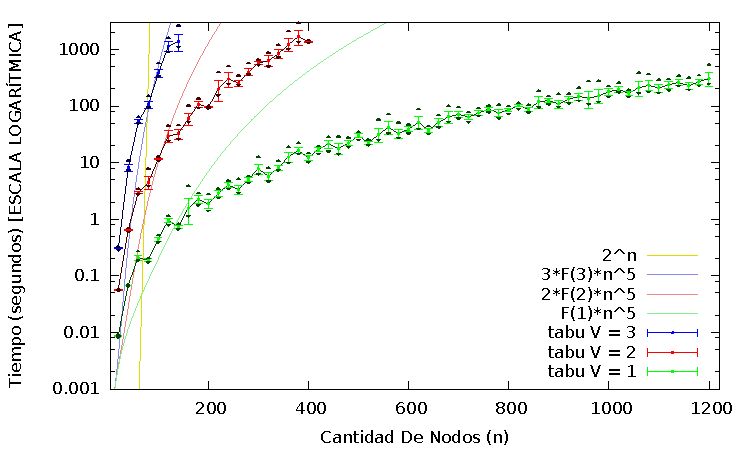
\includegraphics[scale=1.3]{imgs/tabu_1200_20_10.pdf}
\end{center}

\par{Cada punto $\bullet$ en el gráfico representa el promedio de los tiempos
medidos para cada una de las 10 ejecuciones de una determinada cantidad de nodos
del grafo. El tamaño del segmento vertical sobre cada punto $\bullet$ representa
su varianza asociada. Además, para cada cantidad de nodos $n$ se graficaron la
máxima medición con $\blacktriangle$ y la mínima medición con
$\blacktriangledown$.}\\

\par{La función graficada con una curva amarilla es una función exponencial de
base 2. Al estar utilizando escala logarítmica en el eje de ordenadas, esta curva
se ve como una recta. También se graficaron otras tres funciones para que acoten
superiormente cada una de las heurísticas, basándose en su complejidad estimada
en función de $F(V)$. Como se puede observar, si bien incrementando el $V$ los
tiempos de ejecución de la heurística aumentan considerablemente, están muy
lejos de asemejarse a la curva de la función exponencial\footnote{Para que
las comparaciones tengan sentido, las cuatro funciones graficadas fueron
multiplicadas por las mismas constantes. Es por ello que fue difícil ajustar
las tres cotas superiores a las curvas definidas por las tres heurísticas.},
la cual se ve en el gráfico como una recta casi vertical.}

\subsubsection{Optimalidad}

\par{El archivo $opt\_tabu.cpp$ en la carpeta $codigo/tabu$ contiene la
implementación del código que mide el índice de optimalidad de la heurística
de búsqueda tabú. Se ejecutó este programa con\\$N$ = 100\footnote{Para el test
de performance ejecutamos instancias de tamaño 1200. Sin embargo, para calcular
la optimalidad de la heurísica también debemos ejecutar el algoritmo exacto
con cada instancia, lo que nos restringe el máximo tamaño de entrada.},
$s$ = 2 y $k$ = 10. Es decir, para cada $n$ entero par entre 2 y 100, se
generaron 10 grafos aleatorios (con la función $generar\_aristas\_aleatorias$).
Para evaluar como afecta al índice de optimalidad cada uno de los parámetros
($V$ y $T$) por separado, se corrieron para cada parámetro, tres variantes
sobre ese parámetro manteniendo constante el otro. A continuación se
evalúa cada uno por separado. En los test de performance sólo se evaluó la
influencia de $V$ porque ya estaba claro como el valor de $T$
influía sobre la complejidad, no es así sobre el índice de optimalidad.}
\\\\
\textbf{Tamaño de la vecindad $V$}\\

\par{Para cada instancia generada se corrieron las mismas tres variantes que
en el test de performance. Con V=1, con V=2 y con V=3. Para las tres, la
solución inicial fue la solución vacía, tanto el tamaño de la lista tabú
como la cantidad máxima de iteraciones sin mejorar se mantuvieron constantes en
$n$. Para que los datos no se amontonen, utlizamos $s$ = 2 en lugar de $s$ = 1.
En el siguiente gráfico se muestran los resultados obtenidos.}

\begin{center}
\textbf{Gráfico de optimalidad de la heurística de búsqueda tabú
en función\\de la cantidad de nodos del grafo (variando el tamaño de la
vecindad $V$)}
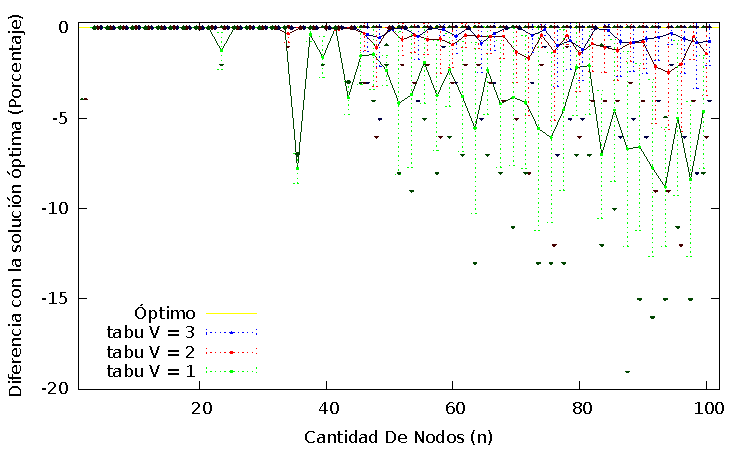
\includegraphics[scale=1.3]{imgs/opt_tabu_100_2_10.pdf}
\end{center}

\par{Cada punto $\bullet$ en el gráfico representa el promedio del índice de
optimalidad para cada una de las 10 ejecuciones de una determinada cantidad de
nodos del grafo. El tamaño del segmento vertical (en líneas punteadas, también
para que los datos no se amontonen) sobre cada punto $\bullet$
representa su varianza asociada. Además, para cada cantidad de nodos $n$ se
graficaron la máxima medición con $\blacktriangle$ y la mínima medición con
$\blacktriangledown$.}\\

\par{La recta $y=0$ representa la solución óptima, así que cuanto más se
asemeje la curva definida por una heurística a dicha recta, mejor es la
heurística. Como se puede observar, para pequeños valores de $n$ las tres
variantes de la heurística encuentran siempre, o casi siempre, una solución
óptima. Al aumentar la cantidad de nodos, aumentan tanto la diferencia
respecto a la solución óptima, como la varianza asociada.}\\

\par{En el caso de la heurística de búsqueda local, la variante con $V$=3 era
claramente superior a las otras dos en cuanto a optimalidad, y las otras dos
eran bastante similares. En el caso de la heurística de búsqueda local es la
variente con $V$=1 la que es claramente distinta (esta vez por ser inferior)
mientras que las variantes con $V$=2 y $V$=3 son bastante similares. En
promedio, la variante con $V$=3 es ligeramente superior, aunque en determinados
casos es inferior a la variante con $V$=2, por lo que no se ve una mejora
considerable por parte de la variante con $V$=3 respecto a la variante
con $V$=2.}\\

\par{Incluso para $n$ mayores, hay instancias para las que las tres variantes de
la heurística encuentran una solución óptima, de hecho para la mayoría de los $n$
hay al menos una instancia para cada variante tal que la variante encuentra
una solución óptima. Esto se ve en los $\blacktriangle$ de las tres variantes
que están sobre la curva $y=0$. Aunque para los mismos $n$ hay instancias en
que la solución devuelta por la variante con $V$=1 difiere en más del 15\% del
óptimo. No es así con las variantes con $V$=2 y $V$=3, cuyos mínimos
en dichos casos difieren en pocos casos en más del 10\% respecto a la solución
óptima. Como esperábamos, la varianza en el índice de optimalidad de la heurística
es muy grande debido a que este depende mucho del tipo de grafo que resuelve.
Al incrementar la cantidad de nodos, las curvas definidas por los resultados de
los algoritmos parecen estabilizarse. En promedio las variantes con $V$=2 y
$V$=3 parecen encontrar soluciones que representan entre el 1\% y el 5\% del
óptimo, mientras que la variante con $V$=1 parece estabilizarse entre el 5\% y
el 10\%. También parece que ninguna de las tres variantes es peor del 20\%.}
\\\\
\textbf{Tamaño de la lista Tabú $T$}\\

\par{Para cada instancia generada se corrieron tres variantes de la heurística.
Con T=$\sqrt{n}$, con T=$n$ y con T=$n^2$. Para las tres, la
solución inicial fue la solución vacía, la cantidad máxima de iteraciones sin
mejorar se mantuvo constante en $n$, mientras que el tamaño de la vecindad se
mantuvo constante en $1$. Para que los datos no se amontonen, utlizamos $s$ = 2
en lugar de $s$ = 1.
En el siguiente gráfico se muestran los resultados obtenidos.}
\newpage
\begin{center}
\textbf{Gráfico de optimalidad de la heurística de búsqueda tabú
en función\\de la cantidad de nodos del grafo (variando el tamaño de la
lista tabú $T$)}
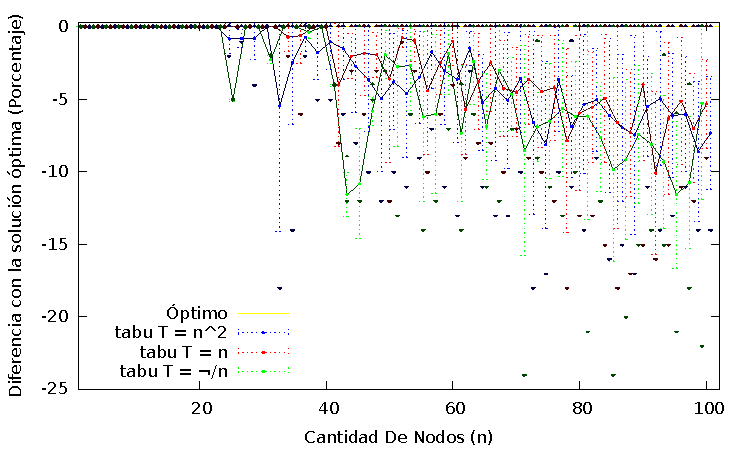
\includegraphics[scale=1.3]{imgs/opt_tabu_T_100_2_10.pdf}
\end{center}

\par{Cada punto $\bullet$ en el gráfico representa el promedio del índice de
optimalidad para cada una de las 10 ejecuciones de una determinada cantidad de
nodos del grafo. El tamaño del segmento vertical (en líneas punteadas, también
para que los datos no se amontonen) sobre cada punto $\bullet$
representa su varianza asociada. Además, para cada cantidad de nodos $n$ se
graficaron la máxima medición con $\blacktriangle$ y la mínima medición con
$\blacktriangledown$.}\\

\par{La recta $y=0$ representa la solución óptima, así que cuanto más se
asemeje la curva definida por una heurística a dicha recta, mejor es la
heurística. Como se puede observar, para pequeños valores de $n$ las tres
variantes de la heurística encuentran siempre, o casi siempre, una solución
óptima. Al aumentar la cantidad de nodos, aumentan tanto la diferencia
respecto a la solución óptima, como la varianza asociada.}\\

\par{En cuanto al parámetro $V$, era claro que incrementarlo producía
mejores resultados. En el caso del parámetro $T$, ninguna de las tres
variantes es claramente superior. Las curvas definidas por ellas se
entrecruzan constantemente, por lo que no es claro cual de las tres
es mejor. Al parecer depende mucho del tipo de grafo entrada y no de
la cantidad de nodos del mismo.}\\

\par{Incluso para $n$ mayores, hay instancias para las que las tres variantes de
la heurística encuentran una solución óptima, de hecho para la mayoría de los $n$
hay al menos una instancia para cada variante tal que la variante encuentra
una solución óptima. Esto se ve en los $\blacktriangle$ de las tres variantes
que están sobre la curva $y=0$. Aunque para los mismos $n$ hay instancias en
que las soluciones difieren en más del 15\% del óptimo. Como esperábamos, la
varianza en el índice de optimalidad de la heurística es muy grande debido a que
este depende mucho del tipo de grafo que resuelve. En este caso no queda claro
que las curvas definidas por los resultados tiendan a estabilizarse al rededor
de un determinado porcentaje de diferencia con el óptimo, pero al menos parece
que ninguna de las tres variantes es peor del 25\%.}

\newpage
\section{Experimentación General}

\par{El objetivo de esta sección es comparar las heurísticas implementadas,
tanto en performance como en optimalidad, entre sí y con el algoritmo exacto.
Los archivos $super\_test.cpp$ y $super\_opt.cpp$ en la carpeta $codigo$
implementan esas pruebas respectivamente. Son iguales a los específicos de cada
heurística pero en lugar de evaluar una sola (o variantes de la misma) evalúa
y compara todas juntas. En cada caso, los algoritmos evaluados fueron los
siguientes:}\\

${\color{yellow}\bullet}$ Algoritmo Exacto con poda\\

${\color{red}\bullet}$ Heurística constructiva golosa\\

${\color{green}\bullet}$ Heurística de búsqueda Local con V=2\\

${\color{cyan}\bullet}$ Heurística de búsqueda Local con V=3\\

${\color{blue}\bullet}$ Heurística de búsqueda Tabú con V=1\\

${\color{violet}\bullet}$ Heurística de búsqueda Tabú con V=2\\

\par{Las heurísticas de búsqueda parten de la solución vacía.
No nos pareció pertinente comparar estos algoritmos con la versión sin
poda del algoritmo exacto ya que sólo servía para compararlo con su contraparte
con poda. No era la idea presentarlo como un algoritmo más, sino que se
implementó para ver que efectivamente la poda disminuía los tiempos de
ejecución. Ya que no hubo mejoras considerables con la heurística de búsqueda
tabú con $V$=3 respecto a su variante con $V$=2\footnote{ver sección
\textbf{experimentación} de \textbf{búsqueda tabú}}, se determinó no evaluar
ambas y, ya que los tiempos de ejecución de la variante con $V$=3 fueron muy
superiores a los de la variante con $V$=2, se eligió esta última.
Tampoco se vieron diferencias considerables al variar el tamaño de la lista $T$
de la búsqueda tabú, por lo que se dejó constante en $n$, al igual que la
cantidad máxima de iteraciones $I$.}\\

\par{Después de
algunas pruebas iniciales se determinó que la heurística de búsqueda local con
$V$=1 era idéntica a la heurística golosa. Tiene sentido si pensamos que
ambas parten de la solución vacía. En cada iteración, la heurística golosa
agrega el nodo que más incrementa la frontera, mientras que búsqueda local,
de las soluciones vecinas a la actual (una solución es vecina si se le agrega o
se le saca un nodo) toma la mejor. Como se parte de la solución vacía, las
soluciones vacinas son todas las que tienen exactamente un nodo, es decir las
mismas que se pueden formar después de la primera iteración de la heurística
golosa.}\\

\par{Para evitar que sean tan similares, se intentó que la solución inicial de
búsqueda local sea la solución de la golosa, pero el problema persistió. Al
parecer, la búsqueda local con $V$=1 no pudo mejorar la solución golosa. Es por
esto que la heurística local con $V$=1 tampoco se evalúa. En el siguiente
gráfico (resultante de ejecutar el programa en $golosa$-$local.cpp$) se ve que
la búsqueda local no puede superar a la golosa ya sea que inicie con la solución
vacía, o con la solución devuelta por la heurística golosa.}
\newpage
\begin{center}
\textbf{Gráfico de optimalidad de las heurísticas golosa y de búsqueda\\
local en función de la cantidad de nodos del grafo}
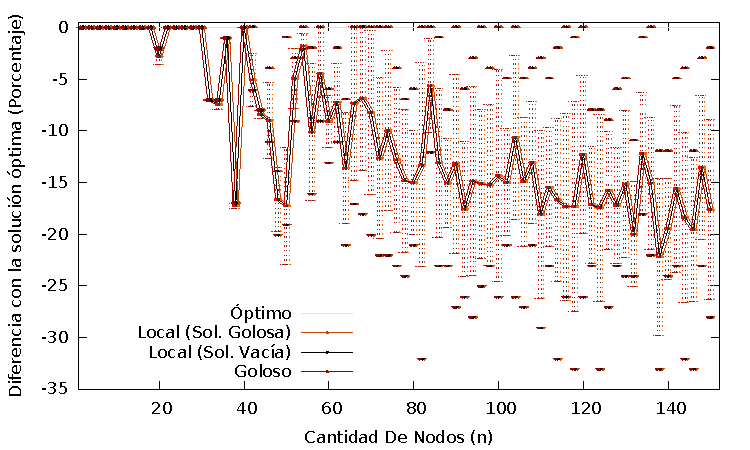
\includegraphics[scale=1.3]{imgs/golosa-local_150_2_10.pdf}
\end{center}

\par{El programa de $golosa-local.cpp$ se corrió con los parámetros $N$ =
150, $s$ = 2 y $k$ = 10. Es decir, para cada $n$ entero par entre 2 y 150, se
generaron 10 grafos aleatorios. Para cada instancia generada se corrieron la
heurística golosa y dos variantes de la búsqueda local con $V$=1. Una a partir
de la solución vacía y otra a partir de la solución obtenida con la heurística
golosa. Como se puede ver, El índice de optimalidad es el mismo para las tres
heurísticas en todos los casos. Incluso coinciden en la varianza, los máximos
y los mínimos.}

\subsection{Performance}

\par{El archivo $super\_test.cpp$ en la carpeta $codigo$ contiene la
implementación del código que mide los tiempos de ejecución de las cinco
heuristicas y del algoritmo exacto. Se ejecutó este programa con $N$ =
150, $s$ = 2 y $k$ = 10. Es decir, para cada $n$ entero par entre 2 y 150, se
generaron 10 grafos aleatorios (con la función $generar\_aristas\_aleatorias$).
Para cada instancia generada se corrieron los seis algoritmos mencionados al
principio de la sección.
En el siguiente gráfico se muestran los resultados obtenidos.}
\newpage
\begin{center}
\textbf{Gráfico de performance general en\\función de la cantidad
de nodos del grafo}
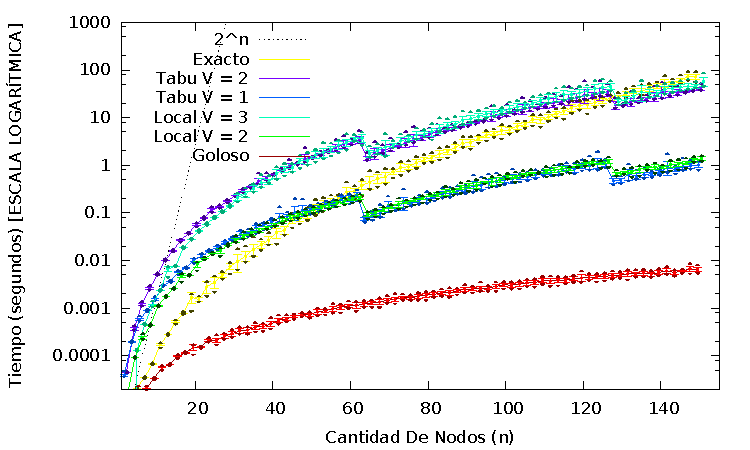
\includegraphics[scale=1.3]{imgs/super_test_150_2_10.pdf}
\end{center}

\par{La curva punteada negra con la etiqueta $2^n$ es la misma que la
graficada en el gráfico de performance del algoritmo exacto, por lo que
debería coincidir más o menos con los tiempos de ejecución de dicho
algoritmo sin poda. Es claro que todas las heurísticas están lejos de alcanzar
tal complejidad.}\\

\par{Debido a los altos tiempos de ejecución del algoritmo exacto (y de las
heurísticas también) nos vimos limitados a testear hasta 150 nodos. A pesar que,
hasta $n$=120 las heurísticas tabú con $V$=2 y local con $V$=3 tienen tiempos de
ejecución superiores al algoritmo exacto, es claro que al incrementar la
cantidad de nodos mucho más, terminará habiendo una mejora considerable (en
cuanto a tiempos de ejecución) de estas heurísticas con respecto al algoritmo
exacto. En este punto ya podemos concluír que para grafos con cantidad de nodos
menor a 120 es preferible usar el algoritmo exacto antes que las heurísticas
tabú con $V$=2 o local con $V$=3, ya que el primero retorna una solución óptima
y tiene menores tiempos de ejecución.}\\

\par{Es notable lo similares que son las curvas definidas por las heurísticas
tabú con $V$=2 y local con $V$=3. En un principio tabú parece ser ligeramente
superior pero a partir de $n$=60, esta pequeña diferencia se invierte. Algo
similar sucede entre las curvas definidas por las heurísticas tabú con $V$=1
y local con $V$=2, donde también la tabú empieza siendo superior, pero luego
pasa a ser inferior a la local.}\\

\par{Otra cosa que llama la atención es la abrupta caída que tienen las cuatro
heurísticas de búsqueda en los grafos con 64 y 128 nodos. Si bien la escala
logarítmica no lo permite ver, esta recaída en los tiempos de ejecución es
de al rededor de la mitad.}

\subsection{Optimalidad}

\par{El archivo $super\_opt.cpp$ en la carpeta $codigo$ contiene la
implementación del código que mide el índice de optimalidad de las cinco
heuristicas. Se ejecutó este programa con $N$ = 150, $s$ = 2 y $k$ = 10. Es
decir, para cada $n$ entero par entre 2 y 150, se generaron 10 grafos
aleatorios (con la función $generar\_aristas\_aleatorias$).
Para cada instancia generada se corrieron los seis algoritmos mencionados al
principio de la sección (Los resultados del algoritmo exacto son siempre
cero. El algoritmo se corre para obtener la máxima frontera de cada instancia
generada y poder calcular el índice de optimalidad de las heurísticas).
En el siguiente gráfico se muestran los resultados obtenidos.}

\begin{center}
\textbf{Gráfico de optimalidad general en\\función de la cantidad
de nodos del grafo}
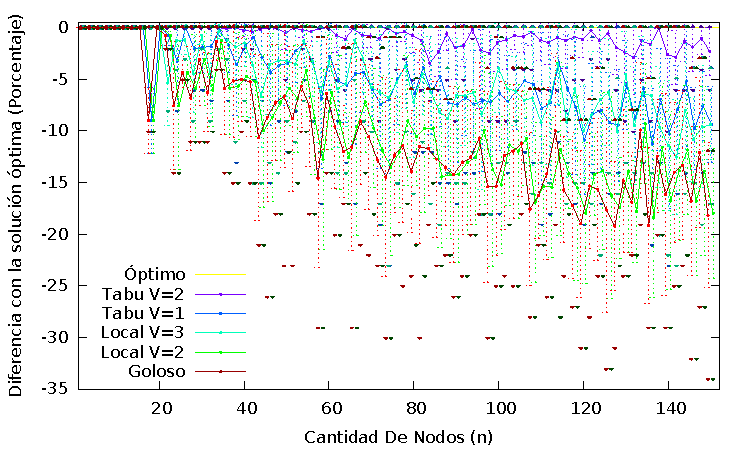
\includegraphics[scale=1.3]{imgs/super_opt_150_2_10.pdf}
\end{center}

\par{Como era de esperarse, la heurística tabú con $V$=2 resultó
ser la más cercana a la recta $y=0$, con un promedio de índice de
optimalidad menor al 5\% y mínimos al rededor del 10\%. Luego le
siguen las heurísticas tabú con $V$=1 y local con $V$=3, con un
promedio de al rededor del 10\% y mínimos entre el 15\% y el 20\%.
Estas dos resultaron ser muy similares en cuanto a optimalidad y
no está del todo claro si alguna es superior a la otra, ya que en
varios puntos se entrelazan. Finalmente, también muy similares entre
sí, las heurísticas golosa y local con $V$=2, con promedios al
rededor del 15\% y mínimos de más del 30\%. El siguiente gráfico
se realizó con los mismos datos pero sin la varianza, además de
reducir el rango vertical para tener una visión más detallada de
las curvas promedio.}
\newpage
\begin{center}
\textbf{Gráfico de optimalidad general en función de\\la cantidad
de nodos del grafo (sin varianza y ampliado)}
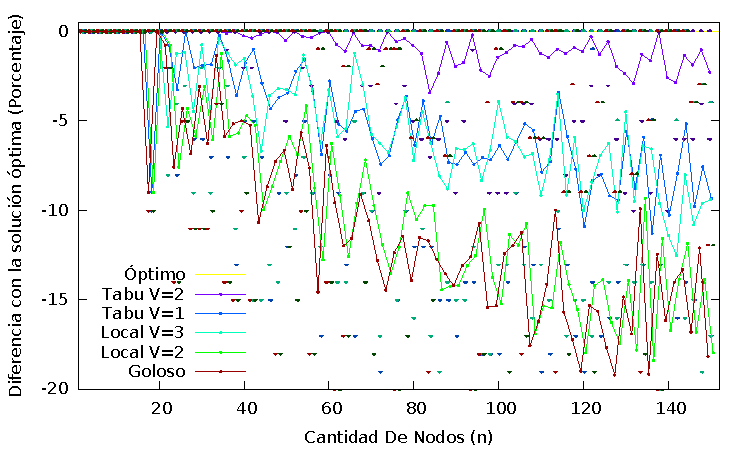
\includegraphics[scale=1.3]{imgs/super_opt_150_2_10_p.pdf}
\end{center}

\par{En este segundo gráfico se pueden observar mejor las relaciones entre las
heurísticas; los segmentos de las varianzas entorpecían mucho la vista y por eso
se decidió quitarlas. A partir de este gráfico y del de performance, podemos
concuír que simepre es mejor utilizar la heurística tabú con $V$=2 antes que la
local con $V$=2, ya que los tiempos de ejecución eran muy similares (de hecho,
la tabú era ligeramente superior a partir de $n$=60) pero la primera obtiene
resultados mucho mejores. Si las opciones son tabú con $V$=1 y local con $V$=3,
también es preferible la opción tabú, ya que ambas tienen resultados similares
pero los tiempos de ejecución de la versión tabú son al menos 10 veces menores
(recordar que el gráfico de performance está en escala logarítmica). Tampoco
es recomendable utilizar la local con $V$=2 frente a la golosa, una vez más
estas dos heurísticas obtienen resultados similares, pero los tiempos de
ejecución de la heurística golosa son muchísimo menores.}\\

\par{Antes de comenzar los tests, se quitó la heurística de búsqueda local con
$V$=1 por ser exactamente igual a la heurística golosa en cuanto a optimalidad.
Sin embargo se ve que su variante con $V$=2 no difiere mucho de la golosa, por
lo tanto tampoco debería diferir mucho de la variante con $V$=1. Si recordamos
el gráfico de optimalidad de búsqueda local\footnote{ver sección
\textbf{experimentación} de \textbf{búsqueda local}} eso es exactamente lo que
sucede.}


\newpage
\section{Conclusiones}
\par{En primera instancia, la realizaci\'on del algoritmo exacto nos sirvi\'o para entender que el conjunto de soluciones
posibles era exponencial sobre la cantidad de nodos del grafo.
Luego comenzamos a implementar las heur\'isticas.}\\

\par{La heur\'istica golosa, fue una primera aproximaci\'on a encontrar una soluci\'on,
no necesariamente \'optima con una cantidad polinomial de operaciones. A pesar de que la idea de la heur\'istica es muy sencilla
(agregar a la soluci\'on nodos que se conecten con la clique actual y que aporten la maxima frontera posible), pudimos obtener una cota
inferior :\\
La frontera siempre ser\'a mayor o igual al grado m\'aximo del grafo.}\\

\par{Con la heur\'istica de búsqueda local pudimos obtener soluciones mejores que las que proporcionaba la golosa (si la vecindad era mayor que 1) con
cierta eficiencia en cuanto a cantidad de operaciones comparado con el algoritmo exacto.}\\

\par{Finalmente con la heurística de búsqeuda tabú, obtuvimos soluciones que generalmente difieren
en un no más de un 10\% de la soluci\'on \'optima ( 5\% si el par\'ametro de vecindad es mayor a 1 ). Esto es gracias a que recorre muchas soluciones
y no para s\'olamente si la soluci\'on es m\'axima de forma local.}\\

\par{Con el trabajo pr\'actico pudimos entender las ideas b\'asicas de las heur\'istcas que son esenciales para problemas en los que los algoritmos exactos
conocidos son exponenciales.}

\newpage
\section{Apéndice}

\subsection {La clase Grafo}
\begin{lstlisting}
struct arista{
	int nodo1;
	int nodo2;
	
	arista(int n, int m){
		this->nodo1 = n;
		this->nodo2 = m;
	}

};

class grafo
public:
 int cantNodos;
 vector< vector<int> > lista_global;
 vector< vector<int> > matriz_ady;
 vector<arista> aristas;

 //Constructor: Construye un grafo vacío
 grafo(){
  grafo(0);
 }

 //Constructor: Construye un grafo con n nodos sin aristas
 grafo(int n){
  constructor(n);
 }

 //Construye el grafo a partir de la entrada estandar
  // (llamar despues del constructor vacío)
 void inicializar() {
  int n, m, a, b, c;
  cin >> n;
  constructor(n);
  if(n != 0) {
   cin >> m;
   for(int i = 0; i < m; ++i){
    cin >> a;
    cin >> b;
    //Paso de 1..n a 0..n-1::
    a--; b--;
    asociar(a,b);
   }
  }
 }

 //Construye un grafo con aristas aleatorias
  // (llamar despues del constructor basico)
 void generar_aristas_aleatorias() {
  srand(time(NULL));
  for(int i = 0; i < cantNodos; ++i)
  for(int j = i; j < cantNodos; ++j)
   if(rand() \%2 == 0) asociar(i, j);
 }

 int gradoMax(){
  unsigned int gradoMax = 0;
  for (int i = 0; i < cantNodos; ++i ){
   if (lista_global[i].size() > gradoMax) {
    gradoMax = lista_global[i].size();
   }
  }
  return gradoMax;
 }

 int grado(int i) {
  return lista_global[i].size();
 }

 void asociar(int nodo1, int nodo2){

  if(nodo1 != nodo2){

   /* Agrego la arista faltante  */
   this->aristas.push_back(arista(nodo1,nodo2));
   
    //agrego cada nodo en la lista del otro nodo incidente
     
    (this->lista_global[nodo1]).push_back(nodo2);
    (this->lista_global[nodo2]).push_back(nodo1);
  
    (this->matriz_ady[nodo1][nodo2]) = 1;
    (this->matriz_ady[nodo2][nodo1]) = 1;
  }
 }
 
 bool hayArista(int nodo1, int nodo2) const{
  return (matriz_ady[nodo2][nodo1] == 1);
 }

 // Devuelve si el nodo 'nodo' se conecta con la clique 'clique'
 bool se_conecta_con_clique(int nodo, vector<bool> &clique){
  for (int i = 0; i < cantNodos; ++i) {
   if ( (clique[i]) && (matriz_ady[i][nodo]==0) ){
    return false;
   }
  }
  return true;
 }

 // Devuelve si el conjunto 'nodos' representa una clique
 bool es_clique(vector<bool> nodos) {
  vector<int> clique = vector<int>();
  for (int i=0; i<cantNodos; i++) {
   if (nodos[i]) {
    for (int j=0; j<clique.size(); j++) {
     if(matriz_ady[i][clique[j]]==0) return false;
    }
    clique.push_back(i);
   }
  }
  return true;
 }

 // Determina cuanto varía la frontera de la clique 'clique'
  // al agregar el nodo 'nodo'
 int cuanto_aporta(int nodo, Solucion &s){
  int frontera_inicial = s.second;
  alternar(s, nodo);
  int frontera_final = s.second;
  alternar(s, nodo);
  return frontera_final - frontera_inicial;
 }

 // Devuelve el v-esimo vecino de la solucion s
 Solucion obtener_vecino(Solucion &s, Solucion &vAnterior, int v) {
  Solucion vecino;
  int nodos_distintos = 1;//Me dice cuantos nodos debo agregar/sacar
  int vecinos = combinatorio(cantNodos,1);
  while (v >= vecinos) {
   nodos_distintos++;
   v -= vecinos;
   vecinos = combinatorio(cantNodos, nodos_distintos);
  }
  if (v==0) {
   vecino = make_pair(s.first, s.second);
   for (int i=0; i<nodos_distintos; i++) {
    alternar(vecino, i);
   }
  } else {
   vecino = make_pair(vAnterior.first, vAnterior.second);
   if (vecino.second < 0) vecino.second*=-1;
   int ov = 0;
   for (int i=cantNodos-1; i>=0; i--) {
    if (s.first[i]!=vAnterior.first[i]) {
     if (i==cantNodos-1-ov) {
      ov ++;
      alternar(vecino, i);
     } else {
      if (ov>0) {
       alternar(vecino, i);
       alternar(vecino, i+1);
       int j = i+2;
       while(ov>0 && j<cantNodos && vecino.first[j]==s.first[j]) {
        alternar(vecino, j);
        j++; ov--;
       }
       if (ov==0) break;								
      } else {
       alternar(vecino, i);
       alternar(vecino, i+1);
       break;
      }
     }
    }
   }
  }
  if (!es_clique(vecino.first)) vecino.second *= -1;
  return vecino;
 }

 void alternar(Solucion &v, int i) {
  v.first[i] = !v.first[i];
  //Recalcular vecino.second (frontera) en funcion del nodo
  // sacado/agregado (no importa si es o no una clique, todavía)
  if (v.first[i]) {
   for (int j=0; j<lista_global[i].size(); j++) {
    if (v.first[lista_global[i][j]]) {
     v.second--;
    } else v.second++;
   }
  } else {
   for (int j=0; j<lista_global[i].size(); j++) {
    if (v.first[lista_global[i][j]]) {
     v.second++;
    } else v.second--;
   }			
  }
 }
 
private:
 void constructor(int n) {
  //cargo la cantidad de nodos
  this->cantNodos = n;

  vector <int> vec;

  //inicializo todas las listas vacias
  for(int i = 0; i < n; i++){
   (this->lista_global).push_back(vector <int>()) ;
  }

  for(int i = 0; i < n; i++){
   (this->matriz_ady).push_back(vector <int>(n)) ;
  }
 }
\end{lstlisting}
\newpage
\subsection{Algoritmo Exacto}

\begin{lstlisting}
Solucion exacto(grafo &g) {
Solucion optima = make_pair(vector<bool>(g.cantNodos,false), 0);
Solucion actual = make_pair(vector<bool>(g.cantNodos,false), 0);
exacto_recur(g, 0, optima, actual);
return optima;
}

Solucion exacto_sin_poda(grafo &g) {
Solucion optima = make_pair(vector<bool>(g.cantNodos,false), 0);
Solucion actual = make_pair(vector<bool>(g.cantNodos,false), 0);
exacto_recur_sp(g, 0, optima, actual);
return optima;
}

void exacto_recur(grafo &g, int i, Solucion &optima, Solucion &actual) {
if (actual.second > optima.second) {
 optima = actual;
}
if (i==g.cantNodos) {
 return;
}

// si se conecta_con_clique sigo la recursion con y sin ese nodo
if ( g.se_conecta_con_clique(i, actual.first) ) {
 g.alternar(actual, i);
 exacto_recur(g, i+1, optima, actual);
 g.alternar(actual, i);
 exacto_recur(g, i+1, optima, actual);
// si no se conecta con mas nodos tampoco va a ser una clique,
// luego hago la recursion sin ese nodo
}else{
 exacto_recur(g, i+1, optima, actual);
}
}

void exacto_recur_sp(grafo &g, int i, Solucion &optima, Solucion &actual) {
if (actual.second > optima.second) {
 optima = actual;
}
if (i==g.cantNodos) {
 return;
}
g.alternar(actual, i);
exacto_recur_sp(g, i+1, optima, actual);
g.alternar(actual, i);
exacto_recur_sp(g, i+1, optima, actual);
}
\end{lstlisting}

\newpage
\subsection{Heur\'istica Golosa}
\begin{lstlisting}
Solucion goloso(grafo g){
Solucion s = make_pair(vector<bool>(g.cantNodos,false), 0);

while (true){
 int candidato = -1;
 int maximo_aporte = 0;

 // veo cual es el nodo que mas aporta y si aporta algo
  // positivo, lo agrego
 for (int i = 0 ; i < g.cantNodos; ++i){				
  if (!s.first[i]){
   if ( g.se_conecta_con_clique(i, s.first) ){
    int aporta = g.cuanto_aporta(i,s);
    if (aporta > maximo_aporte){
     candidato = i;
     maximo_aporte = aporta;
    }
   }
  }
 }

 if (candidato == -1){
  break;
 } else {
  g.alternar(s, candidato);
 }
}

return s;
}

\end{lstlisting}
\newpage
\subsection{Heur\'istica de búsqueda Local}
\begin{lstlisting}
// Parametros:
// * cant_iter: maxima cantidad de iteraciones sin mejorar
// (se reinicia cada vez que mejora)
// * vecinos_size: tamaño de la vecindad
// (cantidad de nodos distintos (como maximo) de cada vecino)
// La cantidad de vecinos en una vecindad de tamaño V es
 // Sum{i=1..V} (n i)
Solucion local(grafo &g, Solucion &sol_inicial, int vecinos_size) {

Solucion sol_actual = make_pair(sol_inicial.first, sol_inicial.second);
bool maximo_local = false;
int vecindad = cant_vecinos(g.cantNodos, vecinos_size);
while (!maximo_local) {
 Solucion sol_mejor = make_pair(vector<bool>(0), -1);//solucion vacia
 //Recorrer vecindad
 Solucion temporal = make_pair(vector<bool>(0), -1);
 for (int i=0; i<vecindad; i++) {
  temporal = g.obtener_vecino(sol_actual, temporal, i);
  if (temporal.second > sol_mejor.second) {
    sol_mejor = temporal;
  }
 }
 if (sol_mejor.second > sol_actual.second) {
  sol_actual = sol_mejor;
 } else {
  maximo_local = true;
 }
}
return sol_actual;
}

\end{lstlisting}
\newpage
\subsection{Metaheur\'istica de búsqeuda Tab\'u}
\begin{lstlisting}
// Parametros:
// * cant_iter: maxima cantidad de iteraciones sin mejorar
// (se reinicia cada vez que mejora)
// * tabu_size: tamaño de la lista tabu
// (cantidad de soluciones que puede almacenar)
// * vecinos_size: tamaño de la vecindad
// (cantidad de nodos distintos (como maximo) de cada vecino)
// La cantidad de vecinos en una vecindad de tamaño V es
// Sum{i=1..V} (n i)
Solucion tabu(grafo &g, Solucion &sol_inicial, int cant_iter, int tabu_size, int vecinos_size) {

Solucion sol_optima = make_pair(sol_inicial.first, sol_inicial.second);
Solucion sol_actual = make_pair(sol_inicial.first, sol_inicial.second);
Tabu_list lista_tabu(tabu_size);
int iter = 0;
int vecindad = cant_vecinos(g.cantNodos, vecinos_size);
while (iter < cant_iter) {
 //solucion vacia
 Solucion sol_mejor = make_pair(vector<bool>(0), -pow(g.cantNodos,2));
 //solucion vacia
 Solucion sol_mejor_tabu = make_pair(vector<bool>(0), -pow(g.cantNodos,2));
 //Recorrer vecindad
 Solucion temporal = make_pair(vector<bool>(0), -1);
 for (int i=0; i<vecindad; i++) {
  temporal = g.obtener_vecino(sol_actual, temporal, i);
  if (temporal.second > sol_optima.second) {
   sol_optima = temporal;
   if (sol_mejor.second > sol_actual.second) iter = -1;
  }
  if (temporal.second > sol_mejor_tabu.second) {
   sol_mejor_tabu = temporal;
  }
  if ((temporal.second > sol_mejor.second)
   &&(!lista_tabu.es_tabu(temporal.first))) {
    sol_mejor = temporal;
  }
 }
 iter++;
 lista_tabu.add_tabu(sol_actual.first);
 sol_actual = sol_mejor;
 // Si no pude tomar ningun vecino valido, tomo una solucion tabu
 if (sol_actual.second==-pow(g.cantNodos,2)) {
  sol_actual = sol_mejor_tabu;
 }
 // Si tampoco tengo una solucion tabu, me quede estancado
 if (sol_actual.second==-pow(g.cantNodos,2)) {
  iter = cant_iter;
 }
}

	return sol_optima;
}

\end{lstlisting}



\end{document}
